\documentclass[doublespace,Afour,sageh,times]{sagej}
\usepackage{amsmath,amssymb,amsthm,mathtools,graphicx,booktabs,array,url,tabularx,multirow}
\usepackage{microtype,etoolbox}
\usepackage{xr-hyper}
\usepackage[colorlinks,bookmarksopen,bookmarksnumbered,citecolor=blue,urlcolor=blue,linkcolor=blue]{hyperref}
\setcounter{secnumdepth}{3}
\setcounter{dbltopnumber}{2}
\renewcommand{\dbltopfraction}{0.90}
\renewcommand{\textfraction}{0.08}
\renewcommand{\floatpagefraction}{0.8}
\emergencystretch=2em
\renewcommand{\bibfont}{\fontsize{9}{11pt}\selectfont}
\setlength{\tabcolsep}{4pt}
\newcolumntype{Y}{>{\raggedright\arraybackslash}X}
\def\journalname{V10 integrated revision}
\def\volumenumber{1}
\def\issuenumber{EN}
\newcommand{\versionlanguage}{English master}
\runninghead{Birkhoff discretization and residual control}
\newtheorem{theorem}{Theorem}
\newtheorem{proposition}[theorem]{Proposition}
\newtheorem{lemma}[theorem]{Lemma}
\newtheorem{corollary}[theorem]{Corollary}
\theoremstyle{definition}
\newtheorem{assumption}{Assumption}
\newtheorem{remark}{Remark}
\newcommand{\R}{\mathbb R}
\newcommand{\C}{\mathbb C}
\newcommand{\T}{\mathbb T}
\newcommand{\dd}{\,\mathrm d}
\newcommand{\norm}[1]{\left\lVert#1\right\rVert}
\newcommand{\abs}[1]{\left|#1\right|}
\newcommand{\diag}{\operatorname{diag}}
\newcommand{\Rea}{\operatorname{Re}}
\newcommand{\Ima}{\operatorname{Im}}
\newcommand{\eps}{\varepsilon}
\providecommand{\doi}[1]{\href{https://doi.org/#1}{doi: #1}.}
\makeatletter
\def\@maketitle{%
\if@Royal
\vspace*{-20pt}
\fi
\if@Crown
\vspace*{-20pt}
\fi
\vspace*{-34pt}%
\null%
\begin{center}
\if@PCfour
\begin{rm}
\else
\begin{sf}
\fi
\begin{minipage}[t]{\textwidth-57.625mm}
  \vskip 12.5pt%
    {\raggedright\titlesize\textbf{\@title} \par}%
    \vskip 1.5em%
    \vskip 12.5mm%
    \end{minipage}\hspace{15mm}\begin{minipage}[t]{42.625mm}
\hbox{}\scriptsize\journalname\\
\hbox{}Direction I framework integration\\
\hbox{}28 October 2026\\
\hbox{}\versionlanguage\\[4pt]
\hbox{}{\fboxsep 2pt\fbox{Research draft}}
\end{minipage}
{\par\large%
\if@Royal
      \vspace*{6mm}
      \fi
      \if@Crown
      \vspace*{6mm}
      \fi%
      \lineskip .5em%
      {\raggedright\textbf{\@author}
      \par}}
     \vskip 40pt%
    {\noindent\usebox\absbox\par}
    {\vspace{20pt}%
      %
      {\noindent\normalsize\@keywords}\par}
      \if@PCfour
      \end{rm}
      \else
      \end{sf}
      \fi
      \end{center}
      \if@Royal
      \vspace*{-4.5mm}
      \fi
      \if@Crown
      \vspace*{-4.5mm}
      \fi
      \vspace{22pt}
        \par%
  }
 
\makeatother


\externaldocument{supplement_xr}[v10_Integrated_EN_Supplement.pdf]
\hypersetup{pdftitle={Birkhoff discretization and complex Hamiltonian residual control of a magnetic catheter model},pdfauthor={Anonymous authors},pdfsubject={V10 and Direction I framework integration, 28 October 2026}}
\begin{document}
\title{Birkhoff discretization and complex Hamiltonian residual control of a magnetic catheter model}
\author{Anonymous authors}
\begin{abstract}
A magnetic catheter model requires a consistent connection between mechanical reduction, learned compensation and numerical dynamics. We develop that connection through three linked subproblems: the matrix implementation of a Birkhoff difference scheme, conservative-residual identification and magnetic realization, and the structure and convergence of the controlled discretization. A planar beam with a tip magnet supplies a common parameter-traceable model, retaining the full coupled cosine potential and endpoint inertia. A compatible time-dependent canonical representation yields a weighted midpoint map, while endpoint projection and noncommuting-matrix elimination make its relation to the ordinary midpoint scheme explicit. Integral state observations identify an analytic potential residual and proportional damping without acceleration labels. The resulting compensation is evaluated inside the same implicit update and realized through magnetic force and torque. We establish finite-time convergence with an explicit accumulated solver-residual term and distinguish it from error relative to the nominal target. When the nonconservative residual is removed, the exactly defined implicit map is exact symplectic. The closed-loop Hamiltonian's quartic normal form and learning-error budget then provide a conditional route to discrete KAM persistence. Linear matrix tests and nonlinear magnetic-control experiments evaluate the three subproblems separately. Full-modal implementation, actuator calibration and a finite-amplitude KAM certificate retain their stated additional requirements.
\end{abstract}
\keywords{Birkhoff systems, magnetic catheter control, residual learning, geometric integration, numerical convergence, discrete KAM}
\maketitle
\raggedbottom
\section{Background and research question}\label{sec:background}
Magnetic actuation applies remote forces and torques to a flexible body through a field and its spatial gradient \citep{abbott,kim}. A useful control model must carry these inputs through mechanical reduction, identification and numerical implementation without changing the dynamical object at each step. This paper studies that chain for a planar clamped--free magnetic catheter model. Negligible gravity motivates the application setting; small slope, no contact and no surrounding-fluid load define the present benchmark. More general rod mechanics remain the starting point for extending these assumptions \citep{simo,antman}.

The nonlinear target retains the complete coupled cosine magnetic potential. Its higher-order terms are not canceled to produce independent linear oscillators: they are the source of the nonlinear frequency variation used in the persistence analysis. The controller compensates an identified conservative residual and proportional damping around that nominal target. The central question is therefore whether the same learned compensation can be connected to a dimensionally correct difference scheme, a physical magnetic command and a precise statement about the resulting discrete dynamics.

\subsection{Three linked subproblems}
\label{fw:three-questions}
\textbf{P1: derive and implement the difference scheme.} Starting from a compatible Birkhoff representation, which endpoint variables admit a generating function, and which matrix update follows? The mechanical mass matrix, phase-flow Jacobian and endpoint transformation have different dimensions. Their distinction matters when a scalar-looking formula is implemented for several modes. Proportional damping also distinguishes a weighted structure-preserving map from ordinary midpoint applied to the damped vector field. We make these constructions explicit and test the noncommuting matrix operations before using the nonlinear catheter model.

\textbf{P2: identify and physically realize residual compensation.} Can state observations determine a conservative residual and damping estimate that preserve the nominal coupled magnetic potential? The identification, controller and simulated plant must use the same coordinates, while the learned controller must not read the unknown coefficients used to generate synthetic data. A second requirement is physical: two generalized modal commands must pass through a common force--torque interface and then a local field--gradient reconstruction. A small identification residual does not by itself verify either sufficient excitation or hardware feasibility.

\textbf{P3: establish the structure and convergence of the controlled scheme.} Once feedback is placed inside the same midpoint equation, which vector field does the scheme approximate, what structure survives identification error, and how does the nonlinear solve affect convergence? The finite-time error must be measured against the same actual closed loop. Its deviation from the nominal target is a separate modeling error. Exact symplecticity is available on the autonomous conservative branch; discrete KAM additionally requires analytic domains, nonresonance, twist and a quantitative smallness condition. These implications cannot be inferred from a phase portrait or a small energy drift.

\subsection{One physical and statistical model throughout}
The benchmark is built from a literature material reference, manufacturer magnet specifications and declared geometric and damping choices. The Sylgard 184 reference is associated with its published formulation and curing conditions \citep{cho2021pdms}; it is not a measurement on the present beam assembly. The tip core contributes translational and rotary inertia before the biased eigenproblem is solved. Those inputs determine the modal scales, physical decoder and magnetic input map used in all three subproblems. Their provenance is given in Section~\ref{sec:derivation} and Supplement~\ref{sec:supp-mechanics}.

The mechanical chain is kept distinct from the learning hypothesis class. Hamiltonian neural networks learn a scalar energy whose derivatives determine a vector field \citep{greydanus}; separate dissipation and actuation terms retain a meaningful power balance \citep{zhong,desai}. Complex coordinates organize the real position and momentum channels, and complex features can supply structured representations \citep{trabelsi}. The real energy depends on a complex coordinate and its conjugate. The analytic continuation required by KAM instead treats the underlying complexified coordinates as independent variables. Neither this notation nor a universal approximation theorem supplies a validated derivative error for an arbitrary fitted network \citep{hornik,zhang}.

The implemented experiment fixes the known kinetic energy and learns an analytic potential residual together with a scalar damping coefficient from integral state observations. It uses a single declared magnetic feature, allowing identification error, numerical error and input reconstruction to be checked separately. A larger analytic readout remains part of the theoretical framework, but the reported computations do not claim unrestricted hidden-layer training or a new complex-versus-real network comparison. The complete nominal cosine is retained even in the single-feature test.

\subsection{Geometric analysis and the control objective}
Generating functions provide established symplectic methods when their geometric and local invertibility assumptions hold \citep{feng,fengqin,hairer}. We use a constructive proportional-damping Birkhoff representation, derive its endpoint projection and time-midpoint update, and recover the ordinary Hamiltonian midpoint map in the conservative limit. The fourth-order central generating function is retained with its complete correction. These classical constructions are applied to the declared mechanical and feedback model; a new general-purpose integration method is not claimed.

The controller estimates damping and a potential correction while retaining $h_0$ as the nominal target. Its actual conservative closed-loop part is $h_c=h_0+\delta R$, where $\delta R$ is the residual identification error. Remaining damping must be retained as a nonconservative term. Consequently, time-discretization convergence can hold when exact symplecticity and classical KAM do not. Section~\ref{sec:analysis} states this separation as a controlled numerical-analysis result, including the accumulated effect of the implicit-solve residual.

The magnetic quartic normal form provides a computable twist for a conditional persistence argument. Learning-to-KAM results require hypotheses beyond a small empirical loss \citep{chen2022}; we therefore retain a deterministic coefficient and analytic-error budget. Continuous KAM offers background for the conservative target \citep{poschel}, while the principal discrete conclusion uses the generating-map framework of \citet{shang}. A finite-amplitude a posteriori certificate would additionally require a specific embedding, invariance defect and geometric bounds \citep{haro2019aposteriori}. Such a new certificate is not supplied by the numerical diagnostics in this study.

Related magnetic-robot studies couple reduced models, visual feedback and simulation to physical control \citep{francescon2025shape,tong2025navigation}. The present contribution isolates the analytical and computational connections needed before those additional sensing and hardware layers are introduced. Learning a conservative reference and tracking it is another valid objective, but it produces a different error system. That related route is retained in Supplement~\ref{sec:supp-tracking}; the main article follows the residual-compensation objective throughout.

\subsection{Contributions and organization}
The first contribution is a complete path from the Birkhoff one-form and endpoint projection to a matrix implementation, with the physical, modal and phase-space dimensions stated explicitly. The second is a shared integral-identification and magnetic-realization construction for residual compensation on the coupled nominal model. The third is an analysis of the controlled discretization that separates finite-time convergence, exact or weighted geometric structure, and conditional discrete KAM persistence. The numerical study is organized to test the corresponding interfaces rather than to combine unrelated accuracy metrics.

\begin{table*}[t]
\centering
\caption{The three subproblems within the six-section article. The same mechanical baseline and compensation objective are retained across the rows.}
\label{tab:roadmap}
\begin{tabularx}{\textwidth}{p{0.15\textwidth}YY}
\toprule
Subproblem & Construction in the article & Verification and limits\\
\midrule
P1: discrete scheme & Section~\ref{sec:derivation}: compatible Birkhoff form, endpoint projection, matrix midpoint and weighted map & Section~\ref{sec:analysis}: independent matrix-exponential references, noncommuting elimination and structure diagnostics\\
P2: learned control & Section~\ref{sec:derivation}: joint integral identification and residual compensation; Section~\ref{sec:application}: physical magnetic ports & Section~\ref{sec:analysis}: four control ablations on one plant; noiseless restricted-feature evidence\\
P3: controlled analysis & Section~\ref{sec:analysis}: feedback inside the implicit scheme and solver-residual convergence; Section~\ref{sec:kam}: discrete persistence conditions & Fixed-model and step-refinement diagnostics; the full analytic KAM budget and device calibration remain separate requirements\\
\bottomrule
\end{tabularx}
\end{table*}

Section~\ref{sec:derivation} supplies the common mechanics and the discrete and learning constructions. Section~\ref{sec:analysis} establishes the controlled scheme's finite-time properties and presents the three-part verification sequence. Section~\ref{sec:kam} connects the conservative branch to discrete KAM. Section~\ref{sec:application} realizes the same command through magnetic ports and states the remaining full-beam and clearance requirements. Section~\ref{sec:conclusion} summarizes the answers to P1--P3. The Supplement provides the detailed proofs, numerical protocols and the related tracking extension.

\section{Mechanical reduction and Birkhoff generating-function construction}\label{sec:derivation}
\subsection{Variational mechanics and the conservative--forced split}
\label{mech:variational}
The residual-compensation construction uses one mechanical object
throughout reduction, identification, discretization and actuation.
We first state the general variational entrance, then specialize it to
a two-mode magnetic beam with known kinetic energy. The coupled
magnetic potential remains in the control target; the learned terms
represent a conservative potential residual and an effective damping
rate. The parameter choices below specify this object and its physical
input scales.

The mechanical starting point is a rod with centreline $r(s,t)$ and
director frame $D(s,t)\in SO(3)$, where $s\in[0,L]$ is reference
arclength. A configuration map $(r(s,q),D(s,q))$ satisfying the essential
boundary conditions and any imposed rod constraints determines both
translational and rotational kinetic energies \citep{simo,antman}.
After spatial reduction, write
\begin{equation}
 T=\tfrac12\dot q^{\mathsf T}M(q)\dot q,\qquad V=V(q),
 \label{mech:general-energy}
\end{equation}
with $M(q)=M(q)^{\mathsf T}\succ0$. Elasticity and a prescribed static
magnetic field contribute to $V$; modulation of that field supplies work.
For a permanent dipole, the interaction potential $-m\cdot B$ gives
$\tau=m\times B$ and $F=\nabla(m\cdot B)$, with orientation held fixed
in the spatial derivative \citep{abbott}.

Let $c_{\rm geo}(q,\dot q)$ be the inertial term generated by derivatives
of $M$, let $\mathcal D_N(q,\dot q)$ be a Rayleigh dissipation potential,
and let $B_u(q)u$ denote the generalized control force. The variational
equations and their Legendre transform are
\begin{align}
 M\ddot q+c_{\rm geo}+\nabla V
 &=Q_{\rm drv}-\partial_{\dot q}\mathcal D_N+B_u u,
 \label{mech:general-lagrange}\\
 p&=M(q)\dot q,\qquad
 H=\tfrac12p^{\mathsf T}M(q)^{-1}p+V,\nonumber\\
 \dot q&=H_p,\qquad v=H_p,\nonumber\\
 \dot p&=-H_q-\partial_v\mathcal D_N(q,v)+Q_{\rm drv}+B_u u.
 \label{mech:general-hamiltonian}
\end{align}
In particular, $(H_q)_i$ contains
$p^{\mathsf T}(\partial_{q_i}M^{-1})p/2$.
The geometric inertia is not an additional dissipative force.
Fluid forcing, moving-boundary work and contact losses can be retained
in $Q_{\rm drv}$ when their models are specified. The derivation in
Supplement~\ref{sm:general} retains these distinctions, including the
fact that a moving fluid can supply mechanical energy. Analytic
persistence results below are restricted to a smooth, contact-free
neighbourhood.

\subsection{A literature-informed physical benchmark}
\label{mech:benchmark}
To obtain a reproducible instance, we specialize this formulation to a
homogeneous circular cantilever in a plane, with a rigid magnetic core
at its distal end. The model has a fixed root and no transverse gravity,
external flow, contact or fluid added mass. This is a gravity-free
mechanical benchmark motivated by remote manipulation, including
microgravity settings; it is not a patient-specific catheter model.
Euler--Bernoulli kinematics neglect shear deformation and distributed
rotary inertia. The tip rotation is approximated by
$\vartheta=w_s(L,t)$; retaining its trigonometric magnetic potential
does not remove this small-slope approximation.

We denote modal damping ratios by $\zeta_j^{\mathrm{d}}$.
Table~\ref{mech:parameters} separates measured material reference
values, nominal magnetic specifications and design choices. The Sylgard
184 reference uses approximately $10$ wt\% curing agent, cured at
$80\,^{\circ}\mathrm C$ for $2$ h \citep{cho2021pdms}. The reported
$E$ and density are approximate reference values for that preparation,
not measurements of the present cylindrical specimen. A $10$ wt\%
curing-agent fraction corresponds to approximately $9{:}1$ base to
curing agent by mass, rather than $10{:}1$.

\begin{table*}[t]
\centering\small
\caption{Inputs to the revised mechanical benchmark. Values designated as
design choices or scenarios are not experimental estimates.}
\label{mech:parameters}
\setlength{\tabcolsep}{5pt}
\begin{tabular}{p{0.27\textwidth}p{0.22\textwidth}p{0.44\textwidth}}
\toprule
Quantity & Value & Basis and interpretation\\
\midrule
Beam length $L$, radius $r$ & $80$ mm, $0.6$ mm & Declared geometry of the uniform solid beam.\\
Young's modulus $E$ & approximately $2.1$ MPa & Sylgard 184 material reference, with the preparation stated in the text \citep{cho2021pdms}.\\
Mass density $\rho$ & approximately $1028\,\mathrm{kg\,m^{-3}}$ & Same material reference \citep{cho2021pdms}; no same-batch specimen calibration is asserted.\\
Bare magnetic-core edge $a_m$ & $0.250$ mm & Declared cubic-core design; coating and adhesive are excluded.\\
Remanent flux density $B_r$ & nominal $1.425$ T & Midpoint of the N50 grade range $1.40$--$1.45$ T \citep{smN50}.\\
Core density $\rho_m$ & nominal $7500\,\mathrm{kg\,m^{-3}}$ & Selected at the manufacturer's stated lower specification; not an individual-core density measurement \citep{smN50}.\\
Axial bias $B_0$ & $30$ mT & Design choice; published OctoMag experiments provide a $40$ mT vector-field capability comparison \citep{lussi2021cvs}.\\
First modal damping ratio $\zeta_1^{\mathrm{d}}$ & $0.025$ & Effective scenario, defined relative to the biased frequency including tip inertia.\\
Effective centreline clearance $c$ & $4$ mm & Design comparison, after subtracting the rod radius from the corridor half-width.\\
\bottomrule
\end{tabular}
\end{table*}

For a uniformly magnetized hard-magnetic core we use the engineering
approximation $\mu\simeq B_ra_m^3/\mu_0$, with
$\mu_0\simeq4\pi10^{-7}\,\mathrm{H\,m^{-1}}$ \citep{kjMoment}.
The nominal dipole moment and inertial properties are
\begin{align}
 \mu&=1.77184214\times10^{-5}\,\mathrm{A\,m^2},\nonumber\\
 m_t=\rho_ma_m^3&=1.171875\times10^{-7}\,\mathrm{kg},\nonumber\\
 J_t=m_ta_m^2/6&=1.220703125\times10^{-15}\,\mathrm{kg\,m^2}.
 \label{mech:core-properties}
\end{align}
The core's centre of mass is idealized at the beam endpoint. An
eccentric installation would introduce inertial coupling and altered
load moment arms. The magnetic-moment estimate does not identify the
magnetization history, coating or manufacturing tolerances of a device.
These assumptions define a consistent numerical object without
combining the material properties of different composite robots.

\subsection{Boundary inertia, finite elements and stored energy}
\label{mech:finite-elements}
Set $A_c=\pi r^2$, $I=\pi r^4/4$, and use the effective damping model
$C=\alpha M_f$. For the associated continuous beam, the interior
equation and clamped boundary are
\begin{align}
 \rho A_cw_{tt}+\alpha\rho A_cw_t+EIw_{ssss}&=0,\nonumber\\
 w(0,t)=w_s(0,t)&=0.
 \label{mech:beam}
\end{align}
Writing $F$ for a transverse tip force and
$\tau_B=\mu B_y\cos\vartheta$ for the active tip torque, the natural
endpoint balances become
\begin{align}
 -EIw_{sss}(L)&=F-m_t[w_{tt}(L)+\alpha w_t(L)],\nonumber\\
 EIw_{ss}(L)&=\tau_B-\mu B_0\sin\vartheta\nonumber\\
 &\quad-J_t(\ddot\vartheta+\alpha\dot\vartheta).
 \label{mech:endpoint-balance}
\end{align}
Thus the terminal rotation remains free. The endpoint damping terms are
part of the declared $C=\alpha M_f$ approximation, not independently
measured losses in the magnetic core.

Let $q$ collect the unconstrained Hermite displacement and slope
coordinates, and let $e_w,e_\vartheta$ select their tip values. The weak
form gives
\begin{align}
 M_f&=M_{\rm beam}+m_te_we_w^{\mathsf T}
                         +J_te_\vartheta e_\vartheta^{\mathsf T},\nonumber\\
 M_f\ddot q+\alpha M_f\dot q+K_{\rm beam}q
 &=e_wF+e_\vartheta(\tau_B-\mu B_0\sin\vartheta),\nonumber\\
 \vartheta&=e_\vartheta^{\mathsf T}q.
 \label{mech:fe-plant}
\end{align}
With $p=M_f\dot q$ and $E_0=\mu B_0$, the nominal physical Hamiltonian is
\begin{align}
 H_0(q,p)&=\tfrac12p^{\mathsf T}M_f^{-1}p
             +\tfrac12q^{\mathsf T}K_{\rm beam}q\nonumber\\
 &\quad+E_0[1-\cos\vartheta].
 \label{mech:fe-energy}
\end{align}
Here $E_0=5.31552642\times10^{-7}\,\mathrm J$.
The bias stores energy, while $F$ and $B_y$ supply work through distinct
physical ports. Their power balance is
\begin{equation}
 \dot H_0=-\alpha\dot q^{\mathsf T}M_f\dot q
              +F\dot w(L)+\tau_B\dot\vartheta.
 \label{mech:physical-power}
\end{equation}

The computation uses $32$ consistent-mass cubic-Hermite elements and
$64$ free nodal coordinates. The independent endpoint characteristic
equation and $16/32/64$-element comparison in
Supplement~\ref{sm:fe-check} verify the first two frequencies to relative
errors $9.02\times10^{-9}$ and $3.29\times10^{-7}$ at $32$ elements.
This checks linear discretization accuracy; the subsequent two-mode
restriction remains a separate model reduction.

\subsection{Mass normalization and canonical scaling}
\label{mech:canonical}
Linearizing the static magnetic term gives
\begin{align}
 K_b&=K_{\rm beam}+E_0e_\vartheta e_\vartheta^{\mathsf T},\nonumber\\
 K_b\Phi_n&=M_f\Phi_n\Omega_n^2,\qquad
 \Phi_n^{\mathsf T}M_f\Phi_n=I_n,
 \label{mech:modal-bias}
\end{align}
where $\Omega_n=\diag(\omega_1,\ldots,\omega_n)$.
With $q=\Phi_na$, the modal momentum is $\pi=\dot a$.
The modal mass is $I_n$ only after this normalization.
Set $\omega_0=\omega_1$, $\tau=\omega_0t$,
$\nu_j=\omega_j/\omega_0$ and $\mathsf N=\diag(\nu_j)$.
The balanced canonical scaling is
\begin{align}
 a_j&=S_jX_j,\qquad S_j=\sqrt{\frac{E_0}{\omega_0\omega_j}},\nonumber\\
 \pi_j&=\sqrt{\frac{E_0\omega_j}{\omega_0}}Y_j,
 \qquad D_s=\diag(S_j).
 \label{mech:scaling}
\end{align}
The position--momentum scale product is $E_0/\omega_0$.
Together with energy $H_0/E_0$ and time $\tau$, this gives canonical
dimensionless equations, rather than a unit-mass replacement of $M_f$.
For the Hermite interpolation row $N_w(s)$, define
\begin{equation}
 \ell(s)^{\mathsf T}=N_w(s)\Phi_nD_s,\qquad
 d=D_s\Phi_n^{\mathsf T}e_\vartheta.
 \label{mech:shape-maps}
\end{equation}
Then $w(s)=\ell(s)^{\mathsf T}X$, $\vartheta=d^{\mathsf T}X$, and
\begin{align}
 h_0(X,Y)&=h_2(X,Y)+g(d^{\mathsf T}X),\nonumber\\
 h_2&=\tfrac12(X^{\mathsf T}\mathsf NX+Y^{\mathsf T}\mathsf NY),\nonumber\\
 g(s)&=1-\cos s-\tfrac12s^2.
 \label{mech:nominal-energy}
\end{align}
The quadratic subtraction avoids counting the bias stiffness twice.
For the two-mode instance,
\begin{align}
 \omega_0&=7.84000916\,\mathrm{rad\,s^{-1}},\nonumber\\
 \nu&=(1,6.04585730)^{\mathsf T},\nonumber\\
 d&=(0.30722439,0.45042632)^{\mathsf T},\nonumber\\
 \ell(L)&=(0.0189673443,0.00775347614)^{\mathsf T}\,\mathrm m.
 \label{mech:reduced-values}
\end{align}
The exported coefficients retain more digits than displayed here.
Additional digits identify the numerical benchmark and do not imply
corresponding measurement precision.
The effective mass in $(X,Y,\tau)$ is $\mathsf N^{-1}$.
Table~\ref{mech:dimension-table} collects the coordinate levels used
by the residual controller and its discretization. The $32$-element
model has $64$ configuration coordinates and a $128$-dimensional phase
space. Restricting its mass-normalized modal family to $n=2$ gives
$I_2$, while the subsequent balanced scaling gives
$M_{\rm eff}=\mathsf N^{-1}$. Each mass belongs to its stated
coordinates. For a general $n$-mode model, the phase-flow Jacobian
$D\Phi$ has size $2n\times2n$, and the joint endpoint transformation
has size $4n\times4n$; in the controlled two-mode system these sizes
are $4\times4$ and $8\times8$. Supplement~\ref{ss:projection}
gives the endpoint projection used by the generating function.

\begin{table*}[t]
\centering\small
\caption{Coordinate levels of the same mechanical benchmark.
Mass normalization and balanced scaling are separate transformations.}
\label{mech:dimension-table}
\setlength{\tabcolsep}{5pt}
\begin{tabular}{p{.22\textwidth}p{.24\textwidth}p{.22\textwidth}p{.23\textwidth}}
\toprule
Level & Coordinates and time & Kinetic mass & Phase-state and tangent sizes\\
\midrule
Complete $32$-element beam & $q,p\in\mathbb R^{64}$, physical $t$ & $M_f\in\mathbb R^{64\times64}$, including $m_t,J_t$ & $128$; $D\Phi\in\mathbb R^{128\times128}$\\
Mass-normalized $n$ modes & $a,\pi\in\mathbb R^n$, physical $t$ & $I_n$; $I_2$ when $n=2$ & $2n$; $D\Phi\in\mathbb R^{2n\times2n}$\\
Balanced two-mode controller & $X,Y\in\mathbb R^2$, $\tau=\omega_0t$ & $M_{\rm eff}=\mathsf N^{-1}$ & $4$; $D\Psi_\Delta\in\mathbb R^{4\times4}$\\
\bottomrule
\end{tabular}
\end{table*}

The damping scenario is
$\alpha=2\zeta_1^{\mathrm{d}}\omega_0=0.3920004581\,\mathrm{s^{-1}}$ and
$\gamma=\alpha/\omega_0=0.05$; it does not assign the same damping ratio
to every mode. Other damping ratios are explored as declared scenarios,
without substituting material loss factors measured under different
conditions for modal damping.

\subsection{Complex coordinates, dissipation and physical inputs}
\label{mech:complex}
Let $x=(X,Y)$ and $J=\left(\begin{smallmatrix}0&I\\-I&0\end{smallmatrix}\right)$.
The invertible complex chart is
\begin{equation}
 \zeta=(X+\mathrm iY)/\sqrt2,\qquad
 \chi=(X-\mathrm iY)/\sqrt2.
 \label{mech:complex-chart}
\end{equation}
On real phase space $\chi=\bar\zeta$. Treating $\zeta,\chi$ as
independent complex variables gives the entire continuation
\begin{equation}
 h_0^{\mathbb C}(\zeta,\chi)
 =\sum_j\nu_j\zeta_j\chi_j
       +g\!\left(d^{\mathsf T}(\zeta+\chi)/\sqrt2\right).
 \label{mech:complex-energy}
\end{equation}
With the convention
$\{\zeta_j,\bar\zeta_k\}=-\mathrm i\delta_{jk}$,
\begin{align}
 \partial_{\bar\zeta}&=(\partial_X+\mathrm i\partial_Y)/\sqrt2,\nonumber\\
 \zeta'&=-\mathrm i\partial_\chi h^{\mathbb C},\qquad
 \chi'=\mathrm i\partial_\zeta h^{\mathbb C}.
 \label{mech:wirtinger}
\end{align}
Analytic continuation in two independent complex arguments is the object
used in analytic KAM theory; a real energy need not be holomorphic in
$\zeta$ alone.

A complex Hamiltonian neural representation supplies a real energy
readout $h_\eta$ and a dimensionless dissipation readout
$\mathcal D_\eta(X,v)$, obtained by dividing physical Rayleigh
dissipation by $E_0\omega_0$. Its dynamics are defined explicitly by
\begin{align}
 X'&=v=\partial_Yh_\eta,\nonumber\\
 Y'&=-\partial_Xh_\eta-\partial_v\mathcal D_\eta(X,v)+U.
 \label{mech:decoder}
\end{align}
The velocity derivative is taken before substituting
$v=\partial_Yh_\eta$. For example,
$\mathcal D_\eta=\widehat\gamma v^{\mathsf T}\mathsf N^{-1}v/2$,
$\widehat\gamma\ge0$, gives
\begin{equation}
 h_\eta'=-v^{\mathsf T}\partial_v\mathcal D_\eta+v^{\mathsf T}U,
 \label{mech:power}
\end{equation}
with $\partial_\tau h_\eta$ added for time-dependent parameters.
Thus $h_\eta+\mathrm i\mathcal D_\eta$ is a pair of decoded readouts,
distinct from the analytic continuation $h_\eta^{\mathbb C}$.
In complex notation the nonconservative term is
$\mathrm i[-\partial_v\mathcal D_\eta+U]/\sqrt2$.

For the fixed-kinetic two-mode model, put
$b_j=e_w^{\mathsf T}\phi_j$, $t_j=e_\vartheta^{\mathsf T}\phi_j$.
The physical input conversion is
\begin{align}
 A_{\rm mag}&=\begin{pmatrix}b_1&t_1\\b_2&t_2\end{pmatrix},
 &\Lambda&=\omega_0^2D_s\mathsf N=E_0D_s^{-1},\nonumber\\
 \Lambda U&=A_{\rm mag}\binom{F}{\tau_B}.
 \label{mech:modal-ports}
\end{align}
A uniform transverse field alone gives
$U=(B_y/B_0)d\cos\vartheta$, a single input direction. Independent
field and gradient authority is needed to realize a general two-vector
$U$. Section~\ref{sec:application} applies this interface to the learned
residual-compensation law and follows the same law into higher-mode
plants. A stronger realization of general target Hamiltonians,
including learned momentum terms, is stated separately in
Supplement~\ref{sm:exact-lift}; the tracking extension uses the shared
interface in Supplementary Section~\ref{sec:supp-tracking}.

\subsection{A compatible Birkhoff representation of the mechanical model}
\label{struct:birkhoff-section}

The first subproblem is to obtain a computable difference scheme from the same mechanical equations that define the catheter. The general model in \eqref{mech:general-hamiltonian} separates the conservative energy, dissipation and applied force. For $z=(q,p)\in\R^{2n}$, a Birkhoff representation uses a one-form $\mathcal R(z,t)^{\mathsf T}\dd z$ and a scalar $\mathcal B$:
\begin{equation}\label{struct:birkhoff}
\begin{aligned}
 \mathcal K_{ij}&=\partial_{z_i}\mathcal R_j-
                  \partial_{z_j}\mathcal R_i,\\
 \mathcal K\dot z&=\nabla_z\mathcal B+\partial_t\mathcal R=:b.
\end{aligned}
\end{equation}
Here $\mathcal K$ must be nonsingular and skew-symmetric. Its entries and $b$ also satisfy
\begin{equation}\label{struct:compatibility}
\begin{aligned}
 \partial_k\mathcal K_{ij}+\partial_i\mathcal K_{jk}
                +\partial_j\mathcal K_{ki}&=0,\\
 \partial_t\mathcal K_{ij}&=\partial_i b_j-\partial_j b_i.
\end{aligned}
\end{equation}
These conditions connect the one-form, scalar and vector field; an arbitrary dissipative force cannot be represented by assigning them independently \citep{su2007}. The Birkhoff matrix is $2n\times2n$, whereas the mass matrix is $n\times n$. Table~\ref{mech:dimension-table} records the dimensions in the finite-element, modal and balanced coordinates. Supplement~\ref{ss:birkhoff} gives the compatibility argument and distinguishes a formal local existence construction from the explicit representation used here.

For proportional momentum damping $\dot p=-H_q-\alpha(t)p$, set $a(t)=\exp\!\int_{t_0}^{t}\alpha(s)\dd s$. A constructive compatible choice is
\begin{equation}\label{struct:weighted-hamiltonian}
\begin{aligned}
 \mathcal R&=(a p,0),\qquad \mathcal B=aH,
       \qquad\mathcal K=-aJ,\\
 \Pi&=a p,\qquad
 \widetilde H(q,\Pi,t)=a(t)H(q,\Pi/a(t),t).
\end{aligned}
\end{equation}
It yields the original equations and makes $Z=(q,\Pi)$ canonical. The construction permits $M=M(q)$ if every mass derivative in $H_q$ is retained. The time dependence of $\widetilde H$ and the return to physical momentum carry the damping; this representation alone does not supply the autonomous conservative system required by classical KAM theory.

\subsection{Endpoint projection and generating-function construction}
\label{struct:endpoint-section}

The endpoint construction and its time expansion play the roles of Theorems A and B in the original framework \citep{feng,fengqin}. We state the local argument needed for the present realization, rather than imposing an inverse on the generated gradient itself. Write $\lambda_Z=\Pi^{\mathsf T}\dd q$. An endpoint transformation $\alpha:(Z_+,Z_-)\mapsto(\widehat w,w)$ is compatible when it is locally invertible and
\[
 \dd(\widehat w^{\mathsf T}\dd w)
      =\dd\lambda_{Z_+}-\dd\lambda_{Z_-}.
\]

\begin{proposition}[Endpoint projection: the role of Theorem A]
\label{struct:endpoint-proposition}
Let $Z_+=\Phi_Z(Z_-)$ be a symplectic graph between fixed time endpoints. Suppose that the compatible transformation $\alpha$ has lower derivative blocks $C_\alpha,D_\alpha$ and
\[
 \det\bigl(C_\alpha D\Phi_Z+D_\alpha\bigr)\ne0.
\]
Then, on a sufficiently small simply connected neighborhood, the graph can be written as $\widehat w=\nabla_w\varphi(w)$. Invertibility of $\partial_w\widehat w$ is not required.
\end{proposition}

\begin{proof}
The stated projection condition makes $w$ a local coordinate on the graph. Symplecticity and compatibility make $\widehat w^{\mathsf T}\dd w$ closed on that graph. The local Poincar\'e lemma then gives the scalar $\varphi$. These steps use the projection onto $w$, not an inverse of its gradient.
\end{proof}

For the central endpoint convention, let $T_0=\diag(I_n,-I_n)$ and $\mathsf E=\left(\begin{smallmatrix}0&I_n\\I_n&0\end{smallmatrix}\right)$. Choose
\begin{equation}\label{struct:endpoint-variables}
\begin{aligned}
 \widehat w&=(\widehat Q,\widehat P)=\mathsf E(Z_+-Z_-),\\
 w&=T_0\bar Z=(Q,P)=(\bar q,-\bar\Pi).
\end{aligned}
\end{equation}
Its full derivative is $4n\times4n$, with $C_\alpha=D_\alpha=T_0/2$. Hence
\begin{equation}\label{struct:endpoint-projection}
 D_{Z_-}w=\tfrac12T_0(D\Phi_Z+I_{2n}).
\end{equation}
At zero step this is $T_0$, so it stays invertible for sufficiently small steps on a fixed compact neighborhood. By contrast, $\widehat w=f(w)$ is identically zero at zero step and $f_w=0$. Supplement~\ref{ss:projection} verifies compatibility, the joint inverse of the endpoint variables and their connection to the Newton matrix.

The role of Theorem B is to turn the time expansion of the endpoint generator into a difference scheme. For the time-dependent Hamiltonian, take the complete temporal midpoint $t_m=t_k+\Delta_t/2$ and use
\begin{equation}\label{struct:lifted-generator}
\begin{aligned}
 \varphi_{\Delta_t}(Q,P)&=-\Delta_t\widetilde H(Q,-P,t_m),\\
 \widehat Q&=-\Delta_t\widetilde H_q(Q,-P,t_m),\\
 \widehat P&=\Delta_t\widetilde H_\Pi(Q,-P,t_m).
\end{aligned}
\end{equation}
Substitution of \eqref{struct:endpoint-variables} gives the canonical time-midpoint equations. For constant $\alpha$ and mass, set $r=\exp(\alpha\Delta_t/2)$ and eliminate the absolute-time exponentials:
\begin{equation}\label{struct:weighted-midpoint}
\begin{aligned}
 q_+-q_-&=\tfrac{\Delta_t}{2}M^{-1}(r p_++r^{-1}p_-),\\
 r p_+-r^{-1}p_-&=-\Delta_t\nabla V\bigl((q_++q_-)/2\bigr).
\end{aligned}
\end{equation}
The exact implicit map obeys
\begin{equation}\label{struct:weighted-structure}
\begin{aligned}
 (D\Phi)^{\mathsf T}J D\Phi&=e^{-\alpha\Delta_t}J,\\
 (D\Phi)^{\mathsf T}\mathcal K(t_+)D\Phi&=\mathcal K(t_-).
\end{aligned}
\end{equation}
This is the pullback of canonical symplecticity in $Z$ through $T_t(q,p)=(q,e^{\alpha t}p)$. Full time-midpoint evaluation gives second-order consistency; freezing explicit time dependence at $t_k$ may leave only first order. For variable mass the same construction applies to the complete $\widetilde H$, but the two constant-mass updates in \eqref{struct:weighted-midpoint} cannot be reused unchanged.

\subsection{The ordinary midpoint scheme and noncommuting matrices}
\label{struct:matrix-section}

The endpoint averages also give an ordinary midpoint discretization of the general physical field:
\begin{equation}\label{struct:mechanical-midpoint}
\begin{aligned}
 q_+-q_-&=\Delta_t M(\bar q)^{-1}\bar p,\\
 p_+-p_-&=\Delta_t[-H_q(\bar q,\bar p)-C_m\bar v]\\
           &\quad+\Delta_t(F_m+U_m),\\
 \bar v&=M(\bar q)^{-1}\bar p.
\end{aligned}
\end{equation}
Every state-dependent quantity is evaluated at the same midpoint and every explicit time argument at $t_m$. This restores the complete vector form of the original matrix update. With general damping it is distinct from \eqref{struct:weighted-midpoint}; second-order accuracy does not imply the exponential structure factor in \eqref{struct:weighted-structure}.

For constant $M,C,K$, with $M\succ0$, $K=K^{\mathsf T}$ and $V(q)=q^{\mathsf T}Kq/2$, elimination of the position midpoint gives
\begin{equation}\label{struct:matrix-elimination}
\begin{aligned}
 E_{\Delta_t}&=\tfrac{\Delta_t^2}{4}KM^{-1}
                         +\tfrac{\Delta_t}{2}CM^{-1},\\
 (I_n+E_{\Delta_t})p_+
    &=(I_n-E_{\Delta_t})p_--\Delta_tKq_-\\
    &\quad+\Delta_t(F_m+U_m),\\
 q_+&=q_-+\tfrac{\Delta_t}{2}M^{-1}(p_++p_-).
\end{aligned}
\end{equation}
The order $KM^{-1}$ follows from substituting $\bar q=q_-+\Delta_tM^{-1}(p_++p_-)/4$ into the momentum equation. No commutation is assumed. Implementation solves the linear system with $I_n+E_{\Delta_t}$, whose invertibility holds for sufficiently small steps. A feedback depending on the unknown midpoint still gives an implicit problem. For $M=M(q)$, the inertial vector $-(\bar p^{\mathsf T}\partial_{q_i}M^{-1}\bar p)/2$ must also be retained; direct solution of the $2n$-dimensional residual is then appropriate. Supplement~\ref{ss:matrix} gives the full elimination.

For the catheter's balanced coordinates, the substitution is
\begin{equation}\label{struct:effective-matrices}
\begin{aligned}
 q&=X,\qquad p=Y,\\
 M_{\rm eff}&=\mathsf N^{-1},\qquad
 C_{\rm eff}=\gamma\mathsf N^{-1}.
\end{aligned}
\end{equation}
Thus $M_{\rm eff}^{-1}Y=\mathsf N Y$ and $C_{\rm eff}M_{\rm eff}^{-1}Y=\gamma Y$. The magnetic force remains nonlinear, so the actual test solves the full residual rather than treating $K$ as a constant replacement for the cosine potential. Section~\ref{sec:analysis} first checks the noncommuting linear algebra against a matrix-exponential reference and then tests the same discretization on that coupled magnetic model.

\subsection{Central generators and the autonomous higher-order extension}
\label{struct:schemes}

For an autonomous Hamiltonian $h$ in $x=(X,Y)$ and dimensionless time $\tau$, write $f=J\nabla h$ and use $\Delta$ for the time step. The central convention is
\begin{equation}\label{struct:central-map}
 x_+-x_-=J\nabla S_\Delta(m),\qquad m=(x_++x_-)/2.
\end{equation}
It is equivalent to the endpoint notation above through $\varphi_\Delta(Q,P)=-S_\Delta(Q,-P)$. The choice $S_\Delta=\Delta h$ gives
\begin{equation}\label{struct:midpoint}
 x_+-x_-=\Delta J\nabla h(m).
\end{equation}
Whenever the implicit equation has a unique local branch, its Jacobian is
\begin{equation}\label{struct:cayley}
 D\Psi_\Delta=(I-C_\Delta)^{-1}(I+C_\Delta),\qquad
 C_\Delta=\tfrac12J S_\Delta''(m).
\end{equation}
Symmetry of $S_\Delta''$ yields symplecticity. With $\lambda=Y^{\mathsf T}\dd X$, the single-valued primitive is
\begin{equation}\label{struct:exact-symplectic}
 \Psi_\Delta^*\lambda-\lambda
 =\dd\bigl[\bar Y^{\mathsf T}(X_+-X_-)-S_\Delta(m)\bigr].
\end{equation}
The map is therefore \emph{exact symplectic}. This stronger property supplies the periodic generating function needed by discrete KAM; it concerns the exact implicit map rather than finite-tolerance solver output.

Retaining the next nonzero term of the central time expansion gives the fourth-order extension \citep{feng}:
\begin{equation}\label{struct:central4}
 S_\Delta^{[4]}(x)=\Delta h(x)
       +\frac{\Delta^3}{24}f(x)^{\mathsf T}h''(x)f(x).
\end{equation}
Supplement~\ref{ss:central4} derives its local $O(\Delta^5)$ defect and harmonic phase formula. The midpoint generator alone remains second order. To obtain a fourth-order controlled method, \eqref{struct:central4} must use all derivatives of the actual autonomous closed-loop Hamiltonian. Adding a separate control increment after a Central4 step does not establish that order or structure.

The principal new-parameter closed-loop calculations use ordinary implicit midpoint on the actual field,
\begin{equation}\label{struct:general-midpoint}
 x_+-x_-=\Delta f_{\rm cl}(m,\tau_m).
\end{equation}
Damping and feedback are evaluated at this same unknown midpoint. A simultaneously integrated reference belongs to the augmented state. Equation~\eqref{struct:midpoint} is the conservative specialization; Section~\ref{sec:analysis} will identify precisely when the controlled field has that form and quantify the effect of an inexact implicit solve. Separate linear and new-parameter nonlinear tests also evaluate Central4 for the conservative target $h_0$, using the explicit derivatives in Supplement~\ref{ss:central4-magnetic-section}. Those fourth-order checks do not assign fourth order or exact symplecticity to a general damped feedback loop.

\subsection{The CHNN model class and the four Hamiltonians}
\label{struct:objects-section}

The complex variables in \eqref{mech:complex-chart} organize the Hamiltonian decoder; the trainable object remains a real energy on the real physical state space. A general CHNN may represent that energy by complex hidden layers followed by a real readout, and may use a separate nonnegative dissipation branch. The force and power equations are then those in \eqref{mech:decoder}--\eqref{mech:power}. The energy and dissipation readouts have different roles: combining their values into one complex output does not make the dissipative dynamics Hamiltonian. Analyticity of the energy on a specified complex neighborhood is an additional requirement for the KAM analysis in Section~\ref{sec:kam}.

To make the identification, force realization and error estimates explicit, the present implementation fixes the known kinetic energy and learns a potential residual. With $\mathsf N=\diag(\nu_1,\nu_2)$ and $\vartheta=d^{\mathsf T}X$, define
\begin{equation}\label{struct:objects}
\begin{aligned}
 g(s)&=1-\cos s-s^2/2,\\
 V_0(X)&=\tfrac12X^{\mathsf T}\mathsf N X+g(d^{\mathsf T}X),\\
 h_0(X,Y)&=\tfrac12Y^{\mathsf T}\mathsf N Y+V_0(X),\\
 h_*&=h_0+R_*,\qquad \widehat h=h_0+\widehat R,\\
 \delta R&=R_*-\widehat R,\qquad h_c=h_0+\delta R.
\end{aligned}
\end{equation}
The four energies are, respectively, the nominal model, the true conservative model within the declared model class, the learned model and the conservative part of the compensation closed loop. They have the same quadratic kinetic energy but different potentials. The actual damped, actuated plant is
\begin{equation}\label{struct:plant}
 X'=\mathsf N Y,\qquad
 Y'=-\nabla(V_0+R_*)(X)-\gamma Y+U.
\end{equation}
An unknown mass, contact force or input gain is not represented by $R_*(X)$; including such effects requires a corresponding model and observation defect.

A finite analytic readout makes the general CHNN architecture directly auditable: $\widehat R(X)=\sum_{j=1}^{m}\widehat\beta_jF_j(X)$ with frozen real analytic features. The minimal experiment takes $m=1$, $F_1=g(d^{\mathsf T}X)$ and an artificial true coefficient $\beta_*=0.2$. This coefficient is an experimental perturbation, not a measured material property. The architecture can retain a complex implementation of these features, but the experiment tests this constrained readout rather than unrestricted hidden-layer training. Supplement~\ref{ss:full-features} gives the full $35$-coefficient quartic readout and explains the additional control requirements when momentum-dependent terms are learned.

\subsection{Joint integral identification of energy and damping}
\label{struct:identification-section}

State observations are divided into disjoint training and validation trajectories. For each observation window $[a_\ell,b_\ell]$, let $c_\ell=(c_{\ell X},c_{\ell Y})$ be an endpoint-matching reconstruction and let $U_\ell^{\rm data}$ be the known input. Set $\mathcal V_F=[\nabla F_1,\ldots,\nabla F_m]$. Integrating the momentum equation gives
\begin{equation}\label{struct:integral-design}
\begin{aligned}
 y_\ell={}&c_{\ell Y}(b_\ell)-c_{\ell Y}(a_\ell)\\
   &+\int_{a_\ell}^{b_\ell}
      [\nabla V_0(c_{\ell X})-U_\ell^{\rm data}]\dd\tau,\\
 D_\ell={}&-\int_{a_\ell}^{b_\ell}
          [\mathcal V_F(c_{\ell X}),c_{\ell Y}]\dd\tau,\\
 \widehat\theta={}&(\widehat\beta_1,\ldots,\widehat\beta_m,
                      \widehat\gamma)^{\mathsf T}.
\end{aligned}
\end{equation}
The stacked design has $nL_I$ rows and $m+1$ columns; here $n=2$, and $L_I$ denotes the number of windows. A QR or SVD solve fits $D\theta\simeq y$ and diagnoses excitation through its singular values. Enforcing $\widehat\gamma\ge0$ gives a passive physical damping estimate. The reproduced calculation uses the unconstrained linear solve, so a negative value at roundoff scale in the zero-damping scenario is reported as a numerical fit result rather than physical negative damping.

No acceleration labels are required. Nevertheless, endpoint noise, interpolation, quadrature and unmodeled dynamics still affect the integrated equation. They enter an independently bounded observation defect, not an inferred consequence of a small training loss. Section~\ref{sec:kam} converts that defect and the Gram lower bound into coefficient, force and analytic energy bounds. The compensation controller and the tracking extension in Supplement~\ref{sec:supp-tracking} use this same frozen fit and the physical input map \eqref{mech:modal-ports}.

\subsection{Residual compensation toward the nominal dynamics}
\label{struct:route-a-section}

The principal controller, denoted Route~A in the reproduced experiments, cancels the estimated damping and potential residual while retaining the complete coupled nominal magnetic energy:
\begin{equation}\label{struct:route-a-control}
 U_A=\widehat\gamma Y+\nabla\widehat R(X).
\end{equation}
Substitution into \eqref{struct:plant}, with $\delta\gamma=\gamma-\widehat\gamma$, yields
\begin{equation}\label{struct:route-a-closed}
 x'=J\nabla h_c(x)+\binom{0}{-\delta\gamma Y}.
\end{equation}
Thus a nonzero conservative learning error changes the closed-loop Hamiltonian to $h_c$; it does not destroy Hamiltonian structure. A nonzero damping error leaves a nonconservative term, with power $h_c'=-\delta\gamma Y^{\mathsf T}\mathsf N Y$. Classical flow or map KAM therefore concerns this physical closed loop only when damping is canceled exactly and the commanded generalized force is realized exactly, or when any remaining force is independently shown to be an autonomous potential gradient and included in $h_c$. A small generic force error is insufficient for this structural premise.

In the exact-compensation limit the closed loop is $h_0$. The nominal reference in the Route~A experiments is the flow of $h_0$ from the same initial state. The oracle uses $U=\gamma Y+\nabla R_*$ solely to separate integration error from identification error; the learned controller uses only the fitted quantities.


The next section inserts this feedback into the same implicit equations and proves the resulting structure and finite-time convergence. Tracking a learned conservative reference is a distinct objective retained in Supplement~\ref{sec:supp-tracking}.

\section{Controlled discretization: convergence and numerical verification}\label{sec:analysis}
\subsection{Putting the feedback into the same implicit equations}
\label{ctrl:placement}

The second subproblem supplies an identified residual and its compensation. The third asks what difference scheme results after that feedback is applied, which structure it preserves, and how its numerical trajectories approach the actual closed-loop dynamics. These questions concern the same plant and the same unknown midpoint used in Section~\ref{sec:derivation}. Substitution of \eqref{struct:route-a-control} into the plant gives the controlled update
\begin{equation}\label{ctrl:midpoint}
\begin{aligned}
 X_+-X_-&=\Delta\mathsf N\bar Y,\\
 Y_+-Y_-&=-\Delta\nabla(V_0+R_*)(\bar X)
               -\Delta\gamma\bar Y\\
        &\quad+\Delta U_A(\bar X,\bar Y)\\
        &=-\Delta\nabla(V_0+\delta R)(\bar X)
               -\Delta\delta\gamma\bar Y.
\end{aligned}
\end{equation}
Thus its continuous target is
$f_c(x)=J\nabla h_c(x)+(0,-\delta\gamma Y)^{\mathsf T}$, including the fixed identification errors. The continuous generalized force $U_A\in\R^2$ is distinguished from its discrete phase-space contribution
\begin{equation}\label{ctrl:control-increment}
 \mathcal U_k=\Delta\binom{0}{U_A(\bar X,\bar Y)}\in\R^4.
\end{equation}
This placement is not generally equivalent to adding a vector after an uncontrolled step or modifying a generating function without deriving its force. The simulated plant contains $R_*$; the feedback evaluates only $\widehat R$ and $\widehat\gamma$. The magnetic input map in Section~\ref{sec:application} must realize this same force for the closed-loop identity to hold.

The Birkhoff construction also has a closed-loop version. For constant residual damping, substitute $\delta\gamma$ and $V_0+\delta R$ into \eqref{struct:weighted-midpoint} and set $r_c=e^{\delta\gamma\Delta/2}$:
\begin{equation}\label{ctrl:weighted-midpoint}
\begin{aligned}
 X_+-X_-&=\tfrac{\Delta}{2}\mathsf N
                  (r_cY_++r_c^{-1}Y_-),\\
 r_cY_+-r_c^{-1}Y_-&=-\Delta\nabla(V_0+\delta R)(\bar X).
\end{aligned}
\end{equation}
When $\delta\gamma=0$, this is exactly \eqref{ctrl:midpoint}. Otherwise its exact map preserves the conformal factor $e^{-\delta\gamma\Delta}$, whereas ordinary midpoint generally does not preserve that exact exponential factor. Equation~\eqref{ctrl:weighted-midpoint} describes a mathematical closed-loop discretization and the specified synthetic comparisons. Implementing its weight requires the residual damping to be specified or independently identified; it does not authorize a learned controller to use unknown plant parameters.

\subsection{The exact structure of the controlled map}
\label{ctrl:structure}

\begin{proposition}[Structure after compensation]
\label{ctrl:structure-proposition}
Suppose the generalized input is realized exactly, the residual energy is twice continuously differentiable, and the implicit branch is locally unique. If $\delta\gamma=0$, the map defined by \eqref{ctrl:midpoint} is exact symplectic, with central generator $S_\Delta^c=\Delta h_c$. If $\delta\gamma$ is constant and nonzero, the exact map of \eqref{ctrl:weighted-midpoint} instead satisfies
\[
 (D\Phi_c)^{\mathsf T}JD\Phi_c=e^{-\delta\gamma\Delta}J.
\]
The latter conclusion is a statement about the weighted scheme, not the ordinary controlled midpoint rule.
\end{proposition}

\begin{proof}
For zero residual damping, \eqref{ctrl:midpoint} is
$x_+-x_-=\Delta J\nabla h_c(\bar x)$. Its tangent is \eqref{struct:cayley} with $C_\Delta=\Delta J\nabla^2h_c/2$. Since $J\nabla^2h_c$ is a Hamiltonian matrix, the Cayley transform preserves $J$. More strongly, \eqref{struct:exact-symplectic} gives
\begin{equation}\label{ctrl:exact-primitive}
 \Psi_c^*\lambda-\lambda
 =\dd[\bar Y^{\mathsf T}(X_+-X_-)-\Delta h_c(\bar x)].
\end{equation}
This single-valued primitive proves exact symplecticity. For nonzero constant residual damping, the canonical lift with
$\Pi=e^{\delta\gamma\tau}Y$ gives \eqref{ctrl:weighted-midpoint}; pulling its symplectic form back to the two time endpoints gives the stated factor. Supplement~\ref{ss:exact-symplectic} supplies the algebra and the periodic action--angle form of the primitive.
\end{proof}

Conservative learning error changes the Hamiltonian from $h_0$ to $h_c=h_0+\delta R$ and is compatible with this exact structure. A damping error is structurally different even if its magnitude is small. If the realized generalized force also has an error $r_U$, then
\begin{equation}\label{ctrl:power}
 h_c'=-(\delta\gamma)Y^{\mathsf T}\mathsf N Y
                         +(\mathsf N Y)^{\mathsf T}r_U.
\end{equation}
An additional error can be included in an autonomous potential only when it has the corresponding gradient structure; on a simply connected position domain, independence of momentum and time and a symmetric position Jacobian are sufficient. Generic input errors, finite Newton residuals and floating-point roundoff have no such guarantee. The KAM result in Section~\ref{sec:kam} therefore concerns the exact conservative implicit map, while the following finite-time convergence result permits a dissipative actual closed loop.

\subsection{Convergence with an algebraic solve residual}
\label{ctrl:convergence-section}

Let $x_c(\tau)$ solve $x'=f_c(x,\tau)$, where $f_c$ includes the fixed feedback, plant parameters and identification errors. This notation also permits a smooth explicit time dependence. Suppose that $f_c$ is twice continuously differentiable on a neighborhood containing the exact and numerical trajectories, with bounded derivatives and a state Lipschitz constant $L_c$. The trajectories and step images have a positive margin from that neighborhood's boundary. For sufficiently small $\Delta$, with $\Delta L_c/2<1$, the local midpoint equation has a unique branch.

A computed step $\widetilde x_k\mapsto\widetilde x_{k+1}$ is allowed to leave the increment residual
\begin{equation}\label{ctrl:solve-residual}
\begin{aligned}
 r_k={}&\widetilde x_{k+1}-\widetilde x_k\\
       &-\Delta f_c((\widetilde x_{k+1}+\widetilde x_k)/2,\tau_m),\\
 &\norm{r_k}\le\eta_k.
\end{aligned}
\end{equation}
Here one fixed vector norm is used consistently. This is the residual of the full increment equation, not the size of a Newton correction. If an implementation reports the infinity norm while trajectory errors use the Euclidean norm, the residual conversion is at most $\sqrt{2n}$; it is $2$ in the two-mode experiment.

\begin{proposition}[Finite-time convergence including the solve residual]
\label{ctrl:convergence}
Under the preceding smoothness, domain and small-step assumptions, let
$e_k=\norm{\widetilde x_k-x_c(\tau_k)}$ and $k\Delta\le T$. There are constants independent of $\Delta$ and of the residual sequence such that
\begin{equation}\label{ctrl:error-recurrence}
\begin{aligned}
 (1-\Delta L_c/2)e_{k+1}
 &\le(1+\Delta L_c/2)e_k\\
 &\quad+C\Delta^3+\eta_k.
\end{aligned}
\end{equation}
If every $\eta_k\le\eta_\Delta$, then
\begin{equation}\label{ctrl:global-error}
 \max_{k\Delta\le T}e_k
 \le C_T\bigl(e_0+\Delta^2+\eta_\Delta/\Delta\bigr).
\end{equation}
More generally, the last term can be replaced by
$\sum_{k\Delta<T}\eta_k$. In particular, per-step residuals
$O(\Delta^3)$ retain second-order convergence.
\end{proposition}

\begin{proof}
Taylor expansion of the exact solution about the temporal midpoint shows that its substitution into the midpoint increment equation leaves a defect bounded by $C\Delta^3$. Subtract that equation from \eqref{ctrl:solve-residual}. The Lipschitz estimate at the two endpoint averages gives
\[
 e_{k+1}\le e_k+\tfrac{\Delta L_c}{2}(e_{k+1}+e_k)
                              +C\Delta^3+\eta_k,
\]
which proves \eqref{ctrl:error-recurrence}. Choose the step range so that $\Delta L_c/2$ stays below a fixed number less than one. The amplification ratio
$(1+\Delta L_c/2)/(1-\Delta L_c/2)$ is then bounded by $1+C_L\Delta$. Iteration over at most $T/\Delta$ steps gives a bounded exponential factor, while the local defects sum to $O(\Delta^2)$ and the algebraic residuals to at most $T\eta_\Delta/\Delta$. This proves \eqref{ctrl:global-error} and its variable-residual version. The domain margin justifies the local equations throughout the comparison; alternatively it can close a small-error continuation argument.
\end{proof}

This result makes the solver tolerance part of the accuracy statement. A fixed absolute tolerance need not sustain a second-order asymptotic rate under indefinite step refinement. The autonomous Central4 method has an analogous estimate
$C_T(e_0+\Delta^4+\eta_\Delta/\Delta)$ when its fifth-order local defect, higher derivative bounds and stable implicit branch hold; a per-step $O(\Delta^5)$ residual preserves fourth order. Supplement~\ref{ss:inexact-solve} records this extension. The residual-budget tests below deliberately perturb increment equations to examine the accumulation term. They are distinguished from the small residuals actually left by Newton iteration.

\subsection{Separating discretization error from compensation error}
\label{ctrl:error-separation}

The exact trajectory in Proposition~\ref{ctrl:convergence} is that of the same actual closed loop, not the nominal trajectory $x_0$ generated by $h_0$. Consequently,
\begin{equation}\label{ctrl:target-error-split}
 \norm{\widetilde x_k-x_0(\tau_k)}
 \le e_k+\norm{x_c(\tau_k)-x_0(\tau_k)}.
\end{equation}
For the same initial state and a common working domain, write
$f_c=f_0+\delta f$, $f_0=J\nabla h_0$, and suppose
$\norm{\delta f}\le\rho_f$ and $f_0$ is $L_0$-Lipschitz there. Gronwall's inequality gives
\[
 \norm{x_c(\tau)-x_0(\tau)}
 \le \rho_f\frac{e^{L_0\tau}-1}{L_0},
\]
with the continuous interpretation $\rho_f\tau$ when $L_0=0$. For exact actuation one may bound
$\rho_f$ by $\sup\norm{\nabla\delta R}+|\delta\gamma|\sup\norm Y$.
Reducing $\Delta$ controls the first term in \eqref{ctrl:target-error-split}; it does not eliminate fixed conservative or damping errors in the second. Independent convergence comparisons therefore use both a reference for $f_c$ and the nominal target, answering different questions.

These results apply to continuous feedback evaluated within the same implicit step. A hardware zero-order hold, a delay or activation of saturation changes the realized field or map. Their errors require the corresponding sampled-control analysis rather than being relabeled as Hamiltonian perturbations. The experiments that follow report the implemented equations, solve residuals and comparison trajectories separately, so that numerical order, compensation quality and geometric structure can each be assessed.


% Generated by reproduction/framework_experiments/build_manuscript_assets.py.
\subsection{Numerical evidence for the three questions}
\label{num:scope}
The experiments follow the three questions in the derivation: P1 checks
the matrix implementation and its stated geometric structure; P2 tests
residual compensation through the physical magnetic ports; P3 separates
convergence to the actual closed field from recovery of a nominal target.
All magnetic calculations use the newly sourced beam and endpoint-core
baseline. The synthetic matrix checks have their own declared,
dimensionless parameters. The reference-tracking extension is retained
in Supplementary Section~\ref{num:route-b}, with its distinct target and
assessment protocol.

Physical-input uncertainty, spatial and modal approximation, coefficient
identification, time integration and feedback error are different sources
of error. Mesh convergence does not measure a two-mode truncation error;
a small integral-fit residual does not bound an analytic norm; and a
small trajectory error does not establish an invariant-torus certificate.
The following tests assign a separate numerical question to each interface.

\subsection{P1: matrix implementation, order and structure}
\label{num:p1}
For $n=1,2,4$, set
\begin{equation}
 \begin{split}
 M&=\operatorname{diag}(1+j/5)_{j=0}^{n-1}
       +0.12\boldsymbol1\boldsymbol1^{\mathsf T},\\
 K&=\operatorname{diag}(1+j)_{j=0}^{n-1}
       +0.05\boldsymbol1\boldsymbol1^{\mathsf T},\qquad C=0.2M.
 \end{split}
 \label{num:matrix-data}
\end{equation}
These are artificial verification matrices, not catheter material
parameters. Each dimension uses a fixed initial state, $T=4$, and steps
$0.08,0.04,0.02,0.01$. Independent matrix exponentials are evaluated at
every point of the finest common time grid. The error is the maximum
Euclidean state error over all saved times, rather than only the endpoint.
For $n=2,4$, $M$ and $K$ do not commute.

The full ordinary-midpoint solve and the correctly ordered eliminated
update agree over their entire trajectories to at most
$5.3959\times10^{-15}$. A second algebraic family uses
$C_g=0.2M+0.03vv^{\mathsf T}/(v^{\mathsf T}v)$, $v=(1,\ldots,n)^{\mathsf T}$.
It checks the order of $C_gM^{-1}$ as well: $C_g$ is nonproportional for
$n=2,4$, while $n=1$ is necessarily a scalar comparison. Its maximum
trajectory discrepancy is $4.6926\times10^{-15}$. No common exponential
weighted-structure claim is assigned to that additional family.

\begin{table*}[t]
\centering
\caption{P1 matrix verification. Orders use full-grid maximum errors at the final step halving. The conservative columns use the quadratic target with stiffness $K+K_s$, $K_s=0.05\operatorname{diag}(1,\ldots,n)$.}
\label{num:matrix-benchmark}
\small
\begin{tabular}{rccccc}
\toprule
$n$ & Max. elimination difference & Ordinary midpoint & Weighted midpoint & Conservative midpoint & Conservative Central4\\
\midrule
1 & $1.144\times10^{-15}$ & $1.999964$ & $1.999942$ & $1.999944$ & $3.999945$ \\
2 & $4.767\times10^{-15}$ & $1.999935$ & $1.999876$ & $1.999890$ & $3.999813$ \\
4 & $5.396\times10^{-15}$ & $1.999869$ & $1.999821$ & $1.999823$ & $3.999864$ \\
\bottomrule
\end{tabular}
\end{table*}

The ordinary damped midpoint and the weighted Birkhoff midpoint both
converge at order two, but their geometric diagnostics differ. At
$n=2$, $\Delta=0.08$, the ordinary map has exponential-weighted defect
$3.9280\times10^{-5}$, whereas the weighted map has defect
$1.1631\times10^{-16}$. Here the defect is
$\|D\Psi^{\mathsf T}JD\Psi-e^{-0.2\Delta}J\|_2$.
For the conservative quadratic target, midpoint and Central4 have
standard symplectic defects at rounding scale and orders two and four,
respectively. The shaping input is exactly specified; no fourth-order
conclusion is assigned to an arbitrary damped feedback update.

The same distinction is checked on the full nonlinear magnetic potential
using the new physical coordinates. For the uncompensated synthetic
plant, ordinary and weighted midpoint have final observed orders
$1.999452$ and $1.999400$ over $0\leq\tau\leq4$.
At $\Delta=0.04$, the ordinary exponential-weighted defect is
$2.8763\times10^{-5}$; the maximum weighted-map defect over all
tested steps is $4.4412\times10^{-16}$. The corresponding known-error
closed-field comparison gives the same structural distinction.
These tests evaluate the implicit ideal tangent at solved numerical
points. They neither establish exact symplecticity of floating-point
Newton code nor give a learning controller access to unknown errors.

\begin{figure*}[t]
\centering
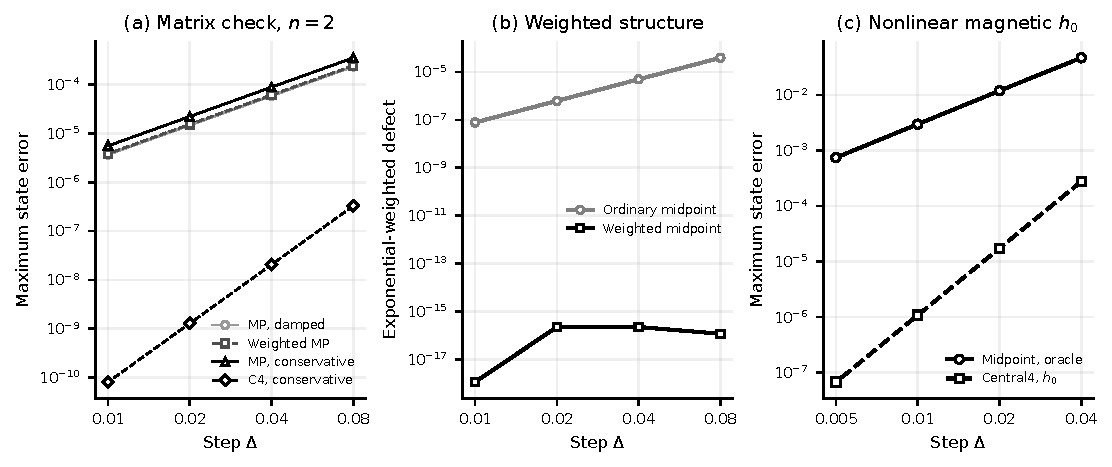
\includegraphics[width=\textwidth]{figures/framework_matrix_checks.pdf}
\caption{P1 checks of the implemented maps. (a) Full-grid matrix errors for $n=2$ against independent matrix exponentials; the damped and conservative groups have their own declared exact targets. (b) Exponential-weighted defects for ordinary and weighted damped midpoint. (c) Midpoint and Central4 on the same nonlinear conservative magnetic $h_0$; these curves compare discretizations of one Hamiltonian. All coordinates, matrices, initial states and reference settings are in the JSON records.}
\label{num:matrix-structure}
\end{figure*}

\subsection{Common physical baseline and modal coordinates}
\label{num:fe}
The benchmark uses the paired material references $E\simeq2.1$ MPa and
$\rho\simeq1028$ kg/m$^3$, with the preparation stated by
\citet{cho2021pdms}. The free length $80$ mm and radius $0.6$ mm are
research design inputs. The nominal $0.250$ mm magnetic cube uses
$B_r=1.425$ T and density $7500$ kg/m$^3$, with their manufacturer-grade
and nominal-selection status retained \citep{smN50,kjMoment}.
Its translational mass and rotary inertia enter the FE mass matrix before
reduction. The consistent $16/32/64$-element frequencies are compared
with independent continuum boundary roots. The largest relative error
among the first four modes is $9.59029\times10^{-6}$ at $32$ elements and
$6.02081\times10^{-7}$ at $64$ elements (Table~\ref{sx:fe-table}).

The adopted $32$-element coordinates are
\begin{align}
 \omega_0=\omega_1&=7.84000916\ \mathrm{rad/s},\notag\\
 \omega_2&=47.39957662\ \mathrm{rad/s},\qquad
 \nu_2=6.04585730,\notag\\
 d&=\bigl(0.30722439,\,0.45042632\bigr)^{\mathsf T},\notag\\
 \ell&=\bigl(0.0189673443,\,0.0077534761\bigr)^{\mathsf T}\ \mathrm m.
 \label{num:scales}
\end{align}
The generator, controls and physical readouts use these same maps.
The declared baseline $C=\alpha M_{\mathrm{total}}$ has
$\zeta_1^{\mathrm d}=0.025$, $\alpha=0.3920004581$ s$^{-1}$ and
$\gamma=0.05$, giving $\zeta_2^{\mathrm d}=0.0041350629$.
These damping ratios are design choices, not measured losses of the
declared beam. Material, inertia and remanence sensitivity points are
reported separately in Table~\ref{sx:sensitivity-table}; they are not
confidence intervals or high-mode control validation.

\subsection{P2: learned residual compensation through the magnetic ports}
\label{num:p2}
\label{num:route-a}
The controlled synthetic departure from $h_0$ is a single potential
feature. Define
\begin{equation}
 \begin{split}
 \phi(X)&=\nabla_X g(d^{\mathsf T}X)\\
        &=d[\sin(d^{\mathsf T}X)-d^{\mathsf T}X],
 \end{split}
 \label{num:feature-gradient}
\end{equation}
and
\begin{equation}
 \begin{split}
 R_*(X)&=\beta_*g(d^{\mathsf T}X),\qquad \beta_*=0.2,\\
 \widehat R(X)&=\widehat\beta g(d^{\mathsf T}X).
 \end{split}
 \label{num:feature}
\end{equation}
The coefficient $0.2$ is a declared stress-test setting, not an identified
material discrepancy. Together with the drag coefficient, this gives a
two-scalar fit. Its recovery does not measure full CHNN optimization or
generalization across richer residual families.

\label{num:identification}
Four training trajectories and two disjoint validation trajectories each
last $\tau=4$. Noiseless states are observed every $0.002$, and Simpson
windows of length $0.04$ produce $400$ training vector increments,
or $800$ scalar rows. For $W=[\tau_a,\tau_b]$ the balance is
\begin{equation}
 \begin{split}
 b_W&=Y_b-Y_a+\int_W\{\mathsf NX+\phi(X)\}\,\mathrm d\tau,\\
 A_W&=\left[-\int_W\phi(X)\,\mathrm d\tau,
                 -\int_WY\,\mathrm d\tau\right],\\
 A_W\binom{\beta}{\gamma}&\simeq b_W.
 \end{split}
 \label{num:regression}
\end{equation}
Column-scaled, unconstrained least squares gives
\begin{equation}
 \widehat\beta=0.200003368491,\qquad
 \widehat\gamma=0.04999999998680.
 \label{num:fitted-values}
\end{equation}
Training and held-out increment RMS residuals are $1.0123\times10^{-12}$ and
$9.2492\times10^{-13}$. The raw and scaled design condition numbers are
$10418.25$ and $1.04537179$. The normalized Gram matrix has
$\lambda_{\min}(G)=5.15486\times10^{-14}$, so weak feature excitation still
matters despite a well-conditioned scaled solve. The truth-dependent
coefficient error $3.36849\times10^{-6}$ is a synthetic diagnostic; an
independently justified integration/observation defect bound remains
necessary for the analytic estimates of Section~\ref{sec:kam}.

All four restoration groups start at
$(0.09,0.08,0.015,-0.01)$ and run to $\tau=20$ ($2.551017$ s),
using midpoint step $0.001$. Every nonzero command is converted to
physical magnetic force/torque and field/gradient, reconstructed and
substituted into the plant during integration. Only the declared oracle
uses true coefficients. Each group is compared with an independently
integrated $h_0$ trajectory from the same initial state.

\begin{table*}[t]
\centering
\caption{P2 restoration through the same physical port map. State and tip RMS use an independent $h_0$ RK4 reference; energy change is the dimensionless nominal quantity $\max_k|h_0(x_k)-h_0(x_0)|$.}
\label{num:a-table}
\begin{tabular}{lccc}
\toprule
Control & State RMS & Tip RMS ($\mu$m) & Maximum nominal energy change\\
\midrule
Passive & $2.92453\times10^{-2}$ & $322.376137$ & $1.50142\times10^{-2}$ \\
Damping compensation & $2.43437\times10^{-5}$ & $0.143531$ & $1.37056\times10^{-7}$ \\
Learned restoration & $1.71438\times10^{-5}$ & $0.094120$ & $5.64520\times10^{-12}$ \\
Oracle restoration & $1.71439\times10^{-5}$ & $0.094120$ & $3.24493\times10^{-12}$ \\
\bottomrule
\end{tabular}
\end{table*}

The fitted restoration reduces the state RMS to $1.71438\times10^{-5}$
and the tip RMS to $0.094120\,\mu$m in this ideal two-mode test.
Its sampled continuous-field mismatch has RMS $2.5942\times10^{-11}$, yet its
trajectory error remains close to the oracle's $1.71439\times10^{-5}$:
both include the same midpoint phase error. A slightly smaller learned
error is compatible with cancellation of two small errors and is not
evidence of outperforming true parameter knowledge. This is restoration
from a shared initial state, not attraction from a tracking offset.

\subsection{P3: convergence to the actual controlled dynamics}
\label{num:p3}
\label{num:integration}
The principal nonlinear oracle midpoint test is retained. Step halvings
$0.04,0.02,0.01,0.005$ give final order $1.999331$ against an
independent RK4 reference, whose step-refinement difference is
$6.3600\times10^{-12}$. A new Central4 test uses the same full-cosine conservative
$h_0$, with all derivatives in Supplementary equation~\eqref{ss:central4-magnetic-jacobian}; it does not append a control
kick after an unrelated map. Its final order is $3.999503$.
The independent DOP853 reference-refinement difference is
$1.1642\times10^{-11}$, below the smallest reported Central4 error.
The analytic increment Jacobian agrees with complex-step differentiation
to $2.7756\times10^{-17}$ at the specified check states.

\begin{table*}[t]
\centering
\caption{Nonlinear conservative $h_0$ integration to $\tau=20$. Errors are maxima over saved times against independent references. Midpoint is the existing perfect-compensation test; Central4 is the new conservative method check.}
\label{num:nonlinear-order}
\begin{tabular}{rcccc}
\toprule
$\Delta$ & Midpoint error & Midpoint order & Central4 error & Central4 order\\
\midrule
$0.04$ & $4.64310\times10^{-2}$ & --- & $2.75432\times10^{-4}$ & --- \\
$0.02$ & $1.18409\times10^{-2}$ & $1.971306$ & $1.73275\times10^{-5}$ & $3.990559$ \\
$0.01$ & $2.96760\times10^{-3}$ & $1.996414$ & $1.08474\times10^{-6}$ & $3.997648$ \\
$0.005$ & $7.42245\times10^{-4}$ & $1.999331$ & $6.78193\times10^{-8}$ & $3.999503$ \\
\bottomrule
\end{tabular}
\end{table*}

To distinguish convergence from model recovery, a separate experiment
freezes the deliberately nonzero identification errors
$\delta\beta=0.02$, $\delta\gamma=0.01$. Thus the controller uses
$\widehat\beta=0.18$, $\widehat\gamma=0.04$ on the same declared plant.
These are manufactured test errors, not outputs of the preceding fit or
measured uncertainty. The actual field is
\begin{equation}
 \begin{split}
 X'&=\mathsf NY,\\
 Y'&=-\mathsf NX-(1+0.02)\phi(X)-0.01Y.
 \end{split}
 \label{num:fixed-error-field}
\end{equation}
The midpoint loop still uses the physical command reconstruction. An
independent DOP853 implementation integrates the explicitly reduced field
above; their sampled field difference is at most $1.1189\times10^{-16}$.
The control coefficients stay frozen for every step size.

\begin{table*}[t]
\centering
\caption{P3 with fixed nonzero identification error. The first error is relative to the same actual continuous closed field; the final column is relative to nominal $h_0$. Both are full-grid maximum Euclidean errors.}
\label{num:closed-convergence}
\begin{tabular}{rccc}
\toprule
$\Delta$ & Error to actual closed field & Observed order & Error to nominal $h_0$\\
\midrule
$0.04$ & $4.20319\times10^{-2}$ & --- & $4.56736\times10^{-2}$ \\
$0.02$ & $1.07152\times10^{-2}$ & $1.971829$ & $1.60584\times10^{-2}$ \\
$0.01$ & $2.68521\times10^{-3}$ & $1.996545$ & $1.17602\times10^{-2}$ \\
$0.005$ & $6.71600\times10^{-4}$ & $1.999364$ & $1.14312\times10^{-2}$ \\
$0.0025$ & $1.67917\times10^{-4}$ & $1.999855$ & $1.14090\times10^{-2}$ \\
\bottomrule
\end{tabular}
\end{table*}

The actual-field error reaches $1.67917\times10^{-4}$ with final order
$1.999855$, while the nominal-target error approaches
$1.14090\times10^{-2}$. Independently integrating the two continuous
models gives a maximum difference $1.14070\times10^{-2}$ on the
finest common grid. Step reduction therefore resolves the actual closed
dynamics but does not eliminate the prescribed modeling error.
The independent reference-refinement difference is $1.0636\times10^{-11}$.
This directly illustrates the scope of the convergence estimate
\eqref{ctrl:global-error}.

\label{num:defect-budget}
A separate one-degree-of-freedom harmonic diagnostic tests its algebraic
residual term. In two-dimensional phase space, we deliberately solve
the perturbed midpoint increment equation with
$r_k=0.01\Delta^q(1,0)^{\mathsf T}$, $q=1,2,3$, over $T=4$.
Every actual original-equation residual is stored. This is a manufactured
algebraic defect, not a measured Newton stopping error or a catheter
experiment. Relative to the unperturbed midpoint trajectory, the added
error has final orders $0.000000,\,1.000000,\,2.000000$; its ratio to
$\eta_\Delta/\Delta$ is approximately $1.999999$.
The total error against the continuous oscillator has final orders
$0.000566,\,1.018776,\,1.999969$, respectively. In particular $q=3$ retains
second order; $q=1$ leaves a nonvanishing error. The test checks the
budget scaling, not a sharp universal value of the theorem's constant.

\begin{figure*}[t]
\centering
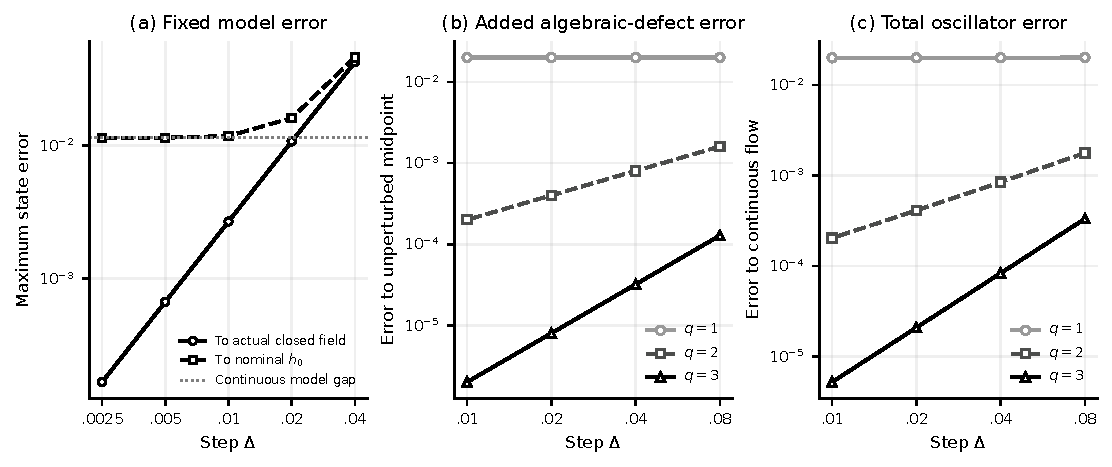
\includegraphics[width=\textwidth]{figures/framework_closed_loop_checks.pdf}
\caption{P3 separates numerical and model errors. (a) With fixed $\delta\beta=0.02$, $\delta\gamma=0.01$, midpoint converges to the actual closed field while its error to $h_0$ approaches the continuous model gap. (b) Added error caused by the manufactured increment defects, measured against unperturbed midpoint. (c) Total error against the independent continuous oscillator; only this diagnostic uses the separate one-degree-of-freedom test model.}
\label{num:closed-results}
\end{figure*}

\subsection{Damping scenarios, sampled domains and remaining boundaries}
\label{num:damping}
The additional ratios $\zeta_1^{\mathrm d}\in\{0,0.01,0.025,0.05,0.1\}$
each receive newly generated training/validation trajectories and a new
fit. Restoration uses $\tau\in[0,10]$, midpoint step $0.002$ and an
independent RK4 reference. Table~\ref{sx:framework-damping-a} reports
passive, learned and oracle groups. This is an in-family sensitivity
study, not one frozen controller resisting unknown damping changes.
The implemented estimator is explicitly unconstrained; it does not
silently implement a nonnegative constrained fit. At zero true damping
it returns $\widehat\gamma=-1.4038\times10^{-12}$, a numerical value that
is not interpreted as negative material loss. Material loss depends on
preparation and frequency and cannot identify these modal ratios without
an additional model or device measurement \citep{fischer2017adhesion}.

\label{num:ports}
The magnetic port matrix has column-normalized condition number
$3.8185963$; its differently dimensioned columns preclude interpreting
a raw condition number as a unit-independent measure.
The principal learned-restoration demands are
$\max|B_y|=0.544490$ mT and
$\max\|\nabla B\|_2=0.01603429$ T/m. Including the longitudinal bias,
the maximum local field is $30.004941$ mT. Published magnetic
systems offer a field-scale comparison \citep{lussi2021cvs}, not a
simultaneous field/gradient feasibility or bandwidth certificate for
these commands. The sampled endpoint angle and whole-beam slope remain
within the declared small-slope diagnostic domain; no continuous-time
or spatial extrema are certified.

No saturation or input-work governor is executed. For a net $4$ mm
clearance, $E_c=10.019717$ nJ and $0.95E_c=9.518731$ nJ,
whereas the principal initial nominal energy is $12.656721$
nJ. The proposed sufficient energy-cap premise is therefore not met
at initialization. The framework tests establish matrix consistency,
specific orders, algebraic port realization and the stated convergence
distinctions. Full-network fitting, higher-mode forced trajectories,
COMSOL comparisons, long-time frequency studies and finite-domain KAM
certificates remain separate tasks. Supplementary
Section~\ref{sx:migration} preserves the status of those earlier results.

\section{Discrete KAM persistence for the compensation dynamics}\label{sec:kam}
\subsection{From nonzero integral loss to a controlled perturbation}
\label{kam:learning-section}

The long-time question concerns the exact implicit map of the compensated catheter. By Proposition~\ref{ctrl:structure-proposition}, this map is exact symplectic when residual damping is zero and the generalized input is realized conservatively. Its Hamiltonian is $h_c=h_0+\delta R$, so the connection to discrete KAM requires a bound on $\delta R$ over a neighborhood, rather than agreement along finitely many trajectories. The nonzero-loss viewpoint of \citet{chen2022} motivates this connection. For the finite readout used here, it can be made deterministic and explicit, without assuming that a training residual vanishes or treating a real-domain prediction error as an analytic norm.

Let $D,y$ be the stacked quantities in \eqref{struct:integral-design}, $\theta_*=(\beta_*^{\mathsf T},\gamma)^{\mathsf T}$ and $e=y-D\theta_*$. Define
\begin{equation}\label{kam:gram}
 G_I=\frac{D^{\mathsf T}D}{nL_I},\qquad
 r_I=\frac{\norm{D\widehat\theta-y}_2}{\sqrt{nL_I}}.
\end{equation}
The defect $e$ includes observation reconstruction, input calibration, quadrature and model-class error. Suppose independent estimates give
$\norm e_2/\sqrt{nL_I}\le\epsilon_I$ and
$\lambda_{\min}(G_I)\ge\underline\lambda>0$ for the matrices actually used. Then
\begin{equation}\label{kam:integral-bound}
 \norm{\widehat\theta-\theta_*}_2
 \le b_I:=\frac{r_I+\epsilon_I}{\sqrt{\underline\lambda}}.
\end{equation}
Indeed, $D(\widehat\theta-\theta_*)=(D\widehat\theta-y)+e$, and the least singular value of $D/\sqrt{nL_I}$ bounds its left-hand side below. This argument applies to any fitted coefficients, including a constrained damping estimate. More observations help only insofar as they improve the defect or the excitation represented by $G_I$.

Let $\mathcal U\subset\C^{2n}$ be a specified complex neighborhood of the real working domain $K$, and define
\begin{equation}\label{kam:feature-bounds}
\begin{aligned}
 B_F(\mathcal U)&=\left(\sum_j\norm{F_j}_{\mathcal U}^{2}\right)^{1/2},\\
 B_{\nabla F}(K)&=\left(\sum_j\sup_K\norm{\nabla F_j}_2^2\right)^{1/2}.
\end{aligned}
\end{equation}
If $R_*=\sum_j\beta_{*,j}F_j+R_{\rm out}$, Cauchy--Schwarz yields
\begin{equation}\label{kam:analytic-error}
\begin{aligned}
 \norm{\delta R}_{\mathcal U}
    &\le b_I B_F(\mathcal U)+\norm{R_{\rm out}}_{\mathcal U},\\
 \sup_K\norm{\nabla\delta R}_2
    &\le b_I B_{\nabla F}(K)+\sup_K\norm{\nabla R_{\rm out}}_2,\\
 |\delta\gamma|&\le b_I.
\end{aligned}
\end{equation}
The first line is an energy perturbation budget for KAM, whereas the second and third enter the tracking equation. Bounds on derivatives over a smaller complex domain also follow from Cauchy estimates, with explicit dependence on the lost domain width. An independently controlled $R_{\rm out}$ must enter both the observation defect and these function bounds. For the synthetic single-feature plant it is zero. The numerical truth-based defect reported in Section~\ref{sec:analysis} is a diagnostic of that experiment; a rigorous or experimental certificate additionally needs validated uncertainty bounds.

\subsection{Real analyticity and the correct complex extension}
\label{kam:analyticity}

The use of complex state coordinates does not by itself supply the analyticity hypothesis. The energy is real on $(X,Y)\in\R^{2n}$, and its extension is holomorphic in the $2n$ independent complex variables $(X,Y)$, or equivalently in independent $(\zeta,\chi)$. On the physical slice $\chi=\bar\zeta$, but this conjugacy is not imposed while taking derivatives in the extended domain. For example,
\begin{equation}\label{kam:complex-energy}
\begin{aligned}
 h_0^{\C}(\zeta,\chi)
  ={}&\sum_j\nu_j\zeta_j\chi_j
      +1-\cos\!\left(\frac{d^{\mathsf T}(\zeta+\chi)}{\sqrt2}\right)\\
     &-\frac{[d^{\mathsf T}(\zeta+\chi)]^2}{4}.
\end{aligned}
\end{equation}
This is the extension of the physical real energy, not a holomorphic function of $\zeta$ alone. Its physical Hamilton equations are obtained by restricting
$\zeta'=-\mathrm i h_\chi^{\C}$ and
$\chi'=\mathrm i h_\zeta^{\C}$ to the real slice.

For a neural readout, every operation must possess a holomorphic continuation on the chosen domain. Polynomial and cosine features meet this requirement. Meromorphic activations require a domain avoiding their poles; piecewise-linear activations do not satisfy this analytic version of KAM. A real part taken at the output is continued by conjugate-symmetric coefficients in the independent variables, not by applying the nonholomorphic real-part operation inside the complex domain. Supplement~\ref{ss:analytic-extension} makes this construction explicit. Both the true residual and the learned residual need the stated regularity. A finitely differentiable KAM theorem is a separate alternative with different differentiability and norm hypotheses; it is not invoked for the present benchmark.

\subsection{A genuine local action--angle model and its twist}
\label{kam:normalform-section}

The balanced variables already diagonalize the positive quadratic energy, $h_2=\tfrac12\sum_j\nu_j(X_j^2+Y_j^2)$. The polar coordinates
$X_j=\sqrt{2I_j}\cos\phi_j$,
$Y_j=-\sqrt{2I_j}\sin\phi_j$
are canonical and give $h_2=\nu\cdot I$. Their radius $I_j$ is not an exact action of the coupled cosine Hamiltonian. A near-identity canonical normal-form transformation is needed before separating an integrable part from a remainder.

To calculate the nominal twist, use $\kappa=1$ in the scalar family $h_\kappa=h_2+\kappa g(d^{\mathsf T}X)$. For this family, the quartic term is $h_{4,\kappa}=-\kappa(d^{\mathsf T}X)^4/24$. Assume
$k\cdot\nu\ne0$ for $0<|k|_1\le4$. The quartic homological equation
\begin{equation}\label{kam:homological}
 \{h_2,W_{4,\kappa}\}
    =-(h_{4,\kappa}-\langle h_{4,\kappa}\rangle)
\end{equation}
has a polynomial solution; the bracket convention is
$\{f,g\}=\nabla f^{\mathsf T}J\nabla g$.
Its local Hamiltonian flow, followed by the polar parametrization on positive actions, defines a canonical chart $\mathcal T_\kappa$. Direct angle averaging gives
\begin{equation}\label{kam:magnetic-twist}
\begin{aligned}
 h_\kappa\circ\mathcal T_\kappa
       &=H_{\rm NF}^{\kappa}(I)+R_6^\kappa(I,\phi),\\
 H_{\rm NF}^{\kappa}(I)
       &=\nu\cdot I+\tfrac12I^{\mathsf T}A_\kappa I,\\
 A_\kappa&=-\frac{\kappa}{8}
 \begin{pmatrix}
 d_1^4&2d_1^2d_2^2\\
 2d_1^2d_2^2&d_2^4
 \end{pmatrix},\\
 \det A_\kappa&=-\frac{3\kappa^2d_1^4d_2^4}{64}.
\end{aligned}
\end{equation}
The off-diagonal terms are essential. The twist is indefinite and nonsingular when $\kappa d_1d_2\ne0$; Kolmogorov nondegeneracy requires invertibility, not positive definiteness. For the new baseline, direct floating-point evaluation gives
$\det A_1\simeq-1.719\times10^{-5}$ and
$\sigma_{\min}(A_1)\simeq2.065\times10^{-3}$. These are reproducible algebraic checks, not interval bounds for a torus. The finite nonresonance check through degree four is also distinct from the all-integer small-divisor condition below.

The remainder is sixth order in Cartesian amplitude because the energy and quartic transformation are even. It includes both the original cosine tail and Poisson-bracket terms generated by the transformation. In particular, $W_{4,\kappa}=\kappa W_{4,1}$ produces terms proportional to $\kappa^2$, so the complete remainder cannot be obtained by multiplying a nominal tail estimate by $\kappa$. Supplement~\ref{ss:normalform} gives this construction and its extension when cubic terms are present.

\subsection{The controlled normal form and its perturbation budget}
\label{kam:closed-budget-section}

The nominal chart $\mathcal T_1$ is built from the same coupled cosine energy that the compensation controller seeks to recover. Applying it to the actual conservative closed loop gives
\begin{equation}\label{kam:closed-budget}
\begin{aligned}
 h_c\circ\mathcal T_1
    &=H_{\rm NF}^{1}(I)+P_c(I,\phi),\\
 P_c&=R_6^{1}+\delta R\circ\mathcal T_1,\\
 \epsilon_c&=\norm{R_6^{1}}_{\mathcal D_c}+b_R^c,\\
 \norm{\delta R\circ\mathcal T_1}_{\mathcal D_c}&\le b_R^c.
\end{aligned}
\end{equation}
Choose a positive action domain $\mathcal I_c\Subset(0,\infty)^2$, its complex action neighborhood and a complex angular strip, collectively denoted $\mathcal D_c$. The chart and its inverse must be analytic with controlled derivatives on the domains being used; their real image must remain in the mechanical working domain. The function bound from \eqref{kam:analytic-error} can be transferred to $b_R^c$ only if the chart image lies inside that same controlled physical complex neighborhood.

Two errors enter \eqref{kam:closed-budget}: the nominal normal-form remainder and the conservative identification error. Even exact identification leaves $R_6^1$, while a small data loss alone bounds neither term. The singular value of $A_1$ computed above establishes an algebraic nondegeneracy check; a finite-amplitude KAM application also needs domain margins, the complete remainder and inverse-chart bounds. The matrix need not be positive definite, but its smallest singular value and inverse norm cannot be omitted from the smallness test.

A learned conservative reference has a different comparison energy: $\widehat h-h_*=-\delta R$, whereas the compensation loop has $h_c-h_0=\delta R$. Supplement~\ref{sec:supp-tracking} retains this distinction and the separate reference-tracking analysis. The principal discrete theorem below concerns $h_c$ and the nominal normal form, without replacing its target by $\widehat h$.

\subsection{Persistence for the actual controlled numerical map}
\label{kam:map-section}

Let $\Psi_\Delta^c$ be the exactly solved map of \eqref{ctrl:midpoint} with $\delta\gamma=0$, or the Central4 map generated from the entire $h_c$. Its analyticity requires a unique implicit branch on a suitable complex neighborhood. One sufficient local condition, together with margins ensuring that the endpoints and images stay inside that neighborhood, is
\begin{equation}\label{kam:implicit-branch}
 \tfrac12\sup\norm{J S_\Delta''}<1.
\end{equation}
For midpoint this is $\Delta\sup\norm{J\nabla^2h_c}/2<1$. It is the same inverse condition that appears in the endpoint projection and Newton matrix in Supplement~\ref{ss:projection}. The exactness proved in \eqref{ctrl:exact-primitive} persists under the analytic canonical normal-form chart, including on the periodic action--angle annulus.

The numerical map to analyze is
$\mathcal T_1^{-1}\circ\Psi_\Delta^c\circ\mathcal T_1$.
It is generally different from applying midpoint after a nonlinear coordinate change. Let
$\mathcal R_\Delta(I,\phi)=(I,\phi+\Delta\omega_0(I))$,
where $\omega_0=\nabla_I H_{\rm NF}^{1}$. On common, suitably reduced analytic domains, local consistency and the flow perturbation estimate give
\begin{equation}\label{kam:map-closeness}
\begin{aligned}
 &\norm{\mathcal T_1^{-1}\Psi_\Delta^c\mathcal T_1
            -\mathcal R_\Delta}\\
 &\qquad\le C_1\Delta\epsilon_c+C_2\Delta^{p+1}.
\end{aligned}
\end{equation}
Here periodic angular lifts are used to compare the maps, and $p=2$ for midpoint or $p=4$ for Central4. The constants require analytic derivative and chart bounds on those domains.

Exact symplecticity and an invertible mixed endpoint projection supply a single-valued periodic generating perturbation $G_\Delta$ relative to $\Delta H_{\rm NF}^{1}$. The domain-reduced estimate is
\begin{equation}\label{kam:map-generator-budget}
 \norm{G_\Delta/\Delta}
       \le C_3\epsilon_c+C_4\Delta^p.
\end{equation}
The normalization by $\Delta$ matters: the per-step generator error is $O(\Delta\epsilon_c+\Delta^{p+1})$, while the smallness quantity in the map theorem is $O(\epsilon_c+\Delta^p)$ \citep[Section~4]{shang}. A smaller step reduces only the discretization part of this budget.

The nonresonance condition is also discrete. The angle increment per step is $\Delta\omega$, and the admissible frequencies satisfy
\begin{equation}\label{kam:map-divisors}
 \left|e^{\mathrm i\Delta k\cdot\omega}-1\right|
       \ge\Delta\gamma_D|k|_1^{-\tau_D},
       \qquad k\in\mathbb Z^2\setminus\{0\}.
\end{equation}
This includes resonances with integer multiples of $2\pi$, so a continuous nonresonance condition or a finite integer scan is insufficient for a chosen step and frequency.

\begin{proposition}[Conditional discrete persistence for the compensated catheter]
\label{kam:map-theorem}
Assume the conservative realization in Proposition~\ref{ctrl:structure-proposition}, real analyticity of the true and learned residuals, the domain and chart bounds in \eqref{kam:closed-budget}, and a unique analytic branch of the exact implicit map. Suppose the nominal frequency map satisfies uniform twist bounds
\[
 \iota\norm v_\infty\le\norm{D_I\omega_0(I)v}_\infty
                \le\Theta\norm v_\infty,
 \qquad0<\iota\le\Theta.
\]
Choose $0<\Delta\le1$, $\tau_D>3$, and
$0<\gamma_D\le\min(1,\rho_I\Theta/2)$,
where $\rho_I$ is the complex action radius. Retain the frequencies satisfying \eqref{kam:map-divisors} at distance at least $2\gamma_D$ from the frequency-domain boundary. If the constants and the reduced analytic domain satisfy the smallness inequality
\begin{equation}\label{kam:map-smallness}
 C_3\epsilon_c+C_4\Delta^p
       \le\delta_0\gamma_D^2\iota^2\Theta^{-3},
\end{equation}
with the $\delta_0$ of the analytic map theorem, then $\Psi_\Delta^c$ has the corresponding Cantor family of invariant quasiperiodic tori. A positive-measure family additionally uses the frequency-domain geometry and measure hypotheses of that theorem.
\end{proposition}

\begin{proof}
The quartic normal form supplies the integrable frequency map and \eqref{kam:closed-budget} bounds its Hamiltonian perturbation. The implicit branch and exact symplecticity give a periodic mixed generating function after conjugation; the consistency estimate gives \eqref{kam:map-generator-budget}. Its smallness and the stated discrete divisors and frequency margins are the analytic hypotheses of \citet[Theorem~2 and Remark~2]{shang}, with the nearly integrable application in that paper's Section~4. Applying the theorem and conjugating the invariant tori back by $\mathcal T_1$ proves the claim. Supplement~\ref{ss:map-kam} records the mixed generating equations and the constants that must be bounded.
\end{proof}

For this affine frequency map, one can take
$\iota=\norm{A_1^{-1}}_\infty^{-1}$ and
$\Theta=\norm{A_1}_\infty$ on the declared domain. Equation~\eqref{kam:map-smallness} states a verification condition; the theorem-dependent constant, complex remainder and chart bounds have not been numerically certified for the present benchmark. No measured training error is substituted for them.

\subsection{Continuous comparison and the scope of the conclusion}
\label{kam:scope}

The continuous Hamiltonian $h_c$ has its own conditional KAM conclusion. It uses the continuous divisors $|k\cdot\omega|\ge\gamma_D|k|_1^{-\tau_D}$ with a permissible exponent $\tau_D>1$ in two degrees of freedom, together with its own analytic smallness conditions \citep{poschel}. Proposition~\ref{kam:flow-theorem} in Supplement~\ref{sec:supp-tracking} states that comparison and its extension to a learned reference. It does not replace the discrete divisor test or identify the continuous tori with those of a chosen numerical map. At a fixed nonzero $\epsilon_c$, letting $\Delta\to0$ does not remove the modeling perturbation or prove convergence of numerical tori to a specified torus of the near-integrable flow.

The present calculations supply the revised physical and modal inputs, the frozen coefficient fit, finite-data diagnostics, the quartic twist and the algebraic structure of the ideal implicit maps. They do not supply an independently certified observation-defect bound, a complete complex normal-form remainder or a numerical evaluation of the KAM threshold. Proposition~\ref{kam:map-theorem} is therefore a conditional result for the benchmark. The learned compensation run retains a nonzero damping error and is not itself declared an exact symplectic map. Its finite-time numerical convergence is instead covered by Proposition~\ref{ctrl:convergence} under that proposition's hypotheses.

A finite-amplitude torus could also be certified by an a posteriori theorem using an approximate embedding, its complex-strip invariance defect, a Diophantine frequency and validated torsion and domain bounds \citep{haro2019aposteriori}. Those quantities require a new calculation for the present parameters; no earlier torus certificate transfers automatically. Invariant tori describe selected bounded discrete motions, not attraction of arbitrary initial states. They also do not establish clearance of the full flexible beam, whose spatial and actuation conditions are treated separately in Section~\ref{sec:application}.

\section{Magnetic realization and whole-beam validation}\label{sec:application}
The application objective is to restore the coupled nominal magnetic
motion through learned residual and damping compensation. The physical
input map must realize the feedback in
\eqref{struct:route-a-control}, preserve its estimation errors and use
the same midpoint convention as \eqref{ctrl:midpoint}. We first close
that chain for the two-mode object, then expose the additional terms
when the same fitted controller acts on more beam modes. The
full-beam clearance argument is a separate condition on physical
energy. Tracking a learned reference is retained as an extension in
Supplementary Section~\ref{sec:supp-tracking}.

\subsection{Magnetic realization of the learned residual compensation}
\label{app:ports}
Use $U=U_A=\widehat\gamma Y+\nabla\widehat R(X)$ from
\eqref{struct:route-a-control} and solve
\begin{equation}
 \binom{F}{\tau_B}=A_{\rm mag}^{-1}\Lambda U.
 \label{app:port-inverse}
\end{equation}
The continuous input $U\in\mathbb R^2$ is dimensionless; $F$ and
$\tau_B$ have units N and N\,m. The four-dimensional discrete increment
in \eqref{ctrl:midpoint} also contains the time step. These conversions
keep the physical force, the continuous generalized input and the
phase-space increment distinct.

Here $\tau_B$ is the active magnetic torque. In the two-mode physical
variables, the synthetic plant used in Section~\ref{sec:analysis} is
\begin{align}
 \ddot a+\alpha\dot a+\Omega_2^2a
 &=\boldsymbol t E_0(\vartheta-\sin\vartheta)
       -\Lambda\nabla R_*(X)\nonumber\\
 &\quad+A_{\rm mag}\binom{F}{\tau_B},
 \qquad a=D_sX.
 \label{app:residual-plant}
\end{align}
Since $\ddot a=\Lambda Y'$ and
$\Lambda\nabla V_0=\Omega_2^2a+\boldsymbol tE_0(\sin\vartheta-\vartheta)$,
substitution recovers \eqref{struct:plant}. A total modal moment is an
equivalent port convention:
\begin{align}
 T&=E_0(\vartheta-\sin\vartheta)+\tau_B,\nonumber\\
 A_{\rm mag}\binom{F}{T}
 &=\Lambda U+\boldsymbol tE_0(\vartheta-\sin\vartheta).
 \label{app:total-port}
\end{align}
The bias-field remainder is known, while the true residual force
$-\Lambda\nabla R_*$ remains in the plant. The controller does not
read $R_*$ through this change of convention.

Substituting the learned law into the physical plant now gives
\begin{align}
 \ddot a&=-\Lambda\nabla V_0
       +(\widehat\alpha-\alpha)\dot a\nonumber\\
       &\quad-\Lambda\nabla\delta R,\nonumber\\
 \widehat\alpha&=\omega_0\widehat\gamma,\qquad
 \delta R=R_*-\widehat R.
 \label{app:physical-closed-loop}
\end{align}
Thus the physical closed loop and
\eqref{struct:route-a-closed} carry the same potential and damping
errors. The compensated target retains the complete coupled nominal
magnetic potential. The truth-only comparator uses known synthetic
parameters solely to separate numerical error from identification
error.

Let the planar dipole be
$m=\mu(\cos\vartheta,\sin\vartheta,0)^{\mathsf T}$.
A local field with the required force and torque is
\begin{align}
 B(r)&=(B_0,B_y,0)^{\mathsf T}+G(r-r_{\rm tip}),\nonumber\\
 B_y&=\frac{\tau_B}{\mu\cos\vartheta},\nonumber\\
 G&=\frac{F}{\mu}
 \begin{pmatrix}
 -\sin\vartheta&\cos\vartheta&0\\
 \cos\vartheta&\sin\vartheta&0\\
 0&0&0
 \end{pmatrix}.
 \label{app:field-gradient}
\end{align}
Direct multiplication gives $Gm=(0,F,0)^{\mathsf T}$ and
$\|G\|_2=|F|/\mu$. Symmetry and zero trace satisfy the local
source-free curl and divergence conditions \citep{abbott}.
The active torque is $\mu B_y\cos\vartheta$; the axial bias torque
$-\mu B_0\sin\vartheta$ remains in the stored-energy model.

Every compensation ablation passes through this same interface.
For the learned group, reconstruct the applied transverse force and active torque from the
field and gradient, and form
\begin{align}
 U_{\rm rec}&=\Lambda^{-1}A_{\rm mag}
                    \binom{F_{\rm app}}{\tau_{B,\rm app}},\nonumber\\
 e_{\rm port}&=U_{\rm rec}-U_A(X,Y).
 \label{app:input-reconstruction}
\end{align}
Ideal exact conversion gives $e_{\rm port}=0$. Calibration errors,
angle-estimation errors, current limits and saturation can make this
quantity nonzero; an input-reconstruction check must retain them in
the applied plant. The reported tests verify the local algebraic
conversion and do not implement saturation.

The interface requires $A_{\rm mag}$ to have rank two, an angle domain
with $|\cos\vartheta|$ bounded away from zero, and feasible joint
field--gradient commands. Column normalization of the nominal matrix
gives condition number $3.8186$, a geometric diagnostic. A physical
authority calculation instead scales the columns by available force
and torque and uses an identified coil-current allocation. A single
uniform field supplies only one modal input direction.

Bias and transverse fields combine as vector magnitudes: a $30$ mT
bias with a $6$ mT transverse component requires $30.594$ mT, whereas
a $20$ mT transverse component requires $36.056$ mT. The published
$40$ mT arbitrary-direction capability of the OctoMag apparatus
\citep{lussi2021cvs} supports this field scale without determining
simultaneous gradient, workspace or bandwidth limits for the present
design. The learned residual-compensation test requires a peak
transverse field of approximately $0.54449$ mT. Section~\ref{sec:analysis}
reports its input reconstruction and sampled operating-domain checks.

\subsection{The same controller on an enriched modal plant}
\label{app:full-model}
Fix the mass-normalized eigenbasis of the $32$-element beam. Retaining
$N\in\{2,4,8,64\}$ modes changes the plant while the fitted two-mode
feedback stays fixed. Write
$a^{(N)}=(a_1,\ldots,a_N)^{\mathsf T}$, and let
$\boldsymbol b_N,\boldsymbol t_N$ collect the corresponding tip
coefficients. Define
\begin{align}
 \vartheta_N&=\boldsymbol t_N^{\mathsf T}a^{(N)},\nonumber\\
 A_{\rm mag}^{(N)}&=[\boldsymbol b_N\ \boldsymbol t_N]
                         \in\mathbb R^{N\times2},\nonumber\\
 X&=D_s^{-1}a_{1:2},\nonumber\\
 Y&=\omega_0^{-1}\mathsf N^{-1}D_s^{-1}\dot a_{1:2}.
 \label{app:enriched-coordinates}
\end{align}
Here $D_s,\mathsf N$ and $A_{\rm mag}$ still denote the fixed low-mode
maps. The first two rows of $A_{\rm mag}^{(N)}$ are $A_{\rm mag}$;
two physical ports cannot independently prescribe all $N$ modal
forces.

A complete conservative residual must now be specified as a physical
potential $\mathcal R_N(a^{(N)})$, measured in joules. The enriched
plant is
\begin{align}
 &\ddot a^{(N)}+\alpha\dot a^{(N)}+\Omega_N^2a^{(N)}\nonumber\\
 &\quad=\boldsymbol t_NE_0(\vartheta_N-\sin\vartheta_N)
       -\nabla_a\mathcal R_N\nonumber\\
 &\qquad+A_{\rm mag}^{(N)}\binom{F_{\rm app}}{\tau_{B,\rm app}}.
 \label{app:enriched-plant}
\end{align}
For a matched synthetic hierarchy, impose
$\mathcal R_N(D_sX,0)=E_0R_*(X)$ by restricting one declared full
potential to each modal subspace. This condition does not identify
that full potential from two-mode data. Supplement~\ref{sm:enriched}
gives explicit extensions and the low-mode projection.

Set $\vartheta_2=d^{\mathsf T}X$ and define the two additional terms
\begin{align}
 e_{\rm mag}^{(N)}
 &=d[\vartheta_N-\sin\vartheta_N\nonumber\\
 &\qquad-\vartheta_2+\sin\vartheta_2],\nonumber\\
 e_R^{(N)}
 &=\Lambda^{-1}\nabla_{a_{1:2}}\mathcal R_N(a^{(N)})\nonumber\\
 &\quad-\nabla R_*(X).
 \label{app:enriched-defects}
\end{align}
With the unchanged learned law, the exact low-mode equations become
\begin{align}
 X'&=\mathsf N Y,\nonumber\\
 Y'&=-\nabla(V_0+\delta R)(X)-\delta\gamma Y\nonumber\\
   &\quad+e_{\rm mag}^{(N)}-e_R^{(N)}+e_{\rm port}.
 \label{app:enriched-closed-loop}
\end{align}
The field conversion uses the actual full angle
$\vartheta=\vartheta_N$; replacing it by a two-mode estimate can also
create $e_{\rm port}$. Even exact port inversion does not eliminate the
high-mode angle or residual differences. A small two-mode training
loss alone therefore supplies neither a truncation bound nor the
Hamiltonian structure needed for the full plant's KAM analysis.

\subsection{A staged full-model validation protocol}
\label{app:staged-validation}
The next validation stages keep the fitted coefficients, low-mode
initial state, reference $h_0$ trajectory and port convention fixed.
The passive, damping-only, learned-compensation and truth-only groups
use the same plant, state information and actuator constraints at each
stage. The truth-only comparator retains its two-mode compensation
law; it is distinct from the stronger full-state feedback described
below. Zero initial high coordinates can still develop a response
because the same two ports act on every retained mode.
Table~\ref{app:validation-stages} separates the completed
numerical check from the proposed enrichments. Mesh convergence in
$16/32/64$ elements checks linear spatial discretization; changing the
number of retained modes checks the forced reduction and controller.

\begin{table*}[t]
\centering\small
\caption{Staged validation of the same fitted residual controller.
The higher-mode and independent finite-element stages are specified
protocols, not newly reported simulation results.}
\label{app:validation-stages}
\begin{tabular}{p{.15\textwidth}p{.45\textwidth}p{.30\textwidth}}
\toprule
Stage & Fixed object and controlled change & Status and required outputs\\
\midrule
Two modes & Fixed-kinetic residual class, one joint fit, common midpoint and magnetic interface & Completed: independent-reference errors, step convergence, reconstruction and sampled demands.\\
$4$ and $8$ modes & Same $32$-element basis, fixed learned law; declared full residual restricted consistently; first zero, then prescribed nonzero high-mode initial conditions & Planned: low-state error, high-mode response and the three defects in \eqref{app:enriched-closed-loop}.\\
All $64$ modes & Same finite-element mass, bias stiffness, core inertia and physical ports; full tip angle used in conversion & Planned: whole-centreline displacement and slope, input peaks, initialization and startup transients.\\
Independent FE model & Rebuild the same geometry, material assumptions, end mass/inertia and boundary loads in COMSOL or an independently specified solver & Planned: verify linear modes first, then compare driven responses and reduction errors under identical input definitions.\\
\bottomrule
\end{tabular}
\end{table*}

Each enriched run should record the full reconstructed centreline,
maximum sampled slope, minimum $|\cos\vartheta_N|$, state RMS error,
tip error, dominant and combination frequencies, force/field/gradient
peaks and saturation fraction. Compare time steps and spatial
extrema within each Hermite element; a plotted tip trace cannot bound
the rest of the beam. Sensor noise, damping mismatch and imposed
limits are introduced in separately declared tests with the same
constraints for every controller. A clipped command is applied to the
plant and included in $e_{\rm port}$, rather than retaining the
unclipped generalized force.

Supplement~\ref{sm:exact-lift} retains a conditional invariant-torus
construction for a stronger exact feedback using known damping and a
target acceleration. That theorem is useful when its full-state
hypotheses can be verified, but it does not replace the unchanged
learned controller in \eqref{app:enriched-closed-loop}. No new
$4/8/64$-mode forced trajectory, COMSOL comparison or finite-amplitude
torus certificate is claimed here.

\subsection{Whole-beam clearance from physical energy}
\label{app:clearance}
Let $E(t)=H_0(q,M_f\dot q)$ be the physical energy of
\eqref{mech:fe-plant}. For every clamped displacement,
\begin{equation}
 w(s)=\int_0^s(s-\xi)w_{ss}(\xi)\dd\xi.
 \label{app:clamped-identity}
\end{equation}
Cauchy--Schwarz and the nonnegative kinetic and bias energies give
\begin{equation}
 \|w\|_\infty^2\le\frac{2L^3E_{\rm bend}}{3EI}
                    \le\frac{2L^3E}{3EI},\qquad
 E_c=\frac{3EIc^2}{2L^3}.
 \label{app:energy-bound}
\end{equation}
Thus $E<E_c$ guarantees clearance of the entire centreline and its
radius tube in the declared straight corridor. The result holds for
arbitrary admissible displacement shapes, including all retained modes;
it is not restricted to a static tip-load shape. For this benchmark,
$E_c=10.0197171$ nJ and the selected cap
$E_{\max}=0.95E_c=9.5187312$ nJ.

An input-work governor can enforce this sufficient condition without
assuming the requested trajectory remains on a torus. Let
$u=(F,B_y)^{\mathsf T}$ and define the physical power coefficient
\begin{equation}
 a_P=\binom{\dot w(L)}{\mu\cos\vartheta\,\dot\vartheta},\qquad
 W(0)\ge E(0),\quad \dot W=a_P^{\mathsf T}u.
 \label{app:work-observer}
\end{equation}
By \eqref{mech:physical-power}, $E(t)\le W(t)$.
Given a request $u_{\rm req}$, choose the closest admissible input in
a scaled positive definite metric $R_u$:
\begin{align}
 u=\mathop{\arg\min}_{\widetilde u\in\mathcal U(q)}
       &\ \tfrac12(\widetilde u-u_{\rm req})^{\mathsf T}
                 R_u(\widetilde u-u_{\rm req}),\nonumber\\
 \text{subject to }&\quad
 a_P^{\mathsf T}\widetilde u\le\kappa(E_{\max}-W),
 \qquad \kappa>0.
 \label{app:work-governor}
\end{align}
Here $\mathcal U(q)$ is a nonempty closed convex feasible joint port set containing zero active
input; $R_u$ accounts for the different force and field units.
If $W(0)<E_{\max}$, zero input is feasible, and
$E_{\max}-W(t)\ge[E_{\max}-W(0)]e^{-\kappa t}>0$.
Together with \eqref{app:energy-bound}, this proves clearance for
solutions satisfying the power identity. Supplement~\ref{sm:work}
extends the argument to specified sensing and execution-error bounds.
For the enriched plant with residual $\mathcal R_N$, the derivative
of the nominal energy also contains
$-\dot a^{(N)\mathsf T}\nabla_a\mathcal R_N$. Its power must be
bounded and included in this ledger, or a separate lower bound of an
augmented energy by bending energy must be proved. The nominal
clearance theorem does not absorb that residual automatically. Activation of the governor can change the requested
Hamiltonian motion, so the clearance proof is distinct from torus
preservation.

The reported residual-compensation tests do not use this governor.
Their nominal-reference initial state has energy $12.6567$ nJ, already
above the $9.5187$ nJ cap.
Consequently, the observed displacement and slope maxima in
Section~\ref{sec:analysis} are numerical operating-domain diagnostics,
not consequences of this energy-cap guarantee. The governor supplies
a precise condition for a future full-state experiment initialized
inside the admissible energy set.

\section{Conclusion}\label{sec:conclusion}
The three subproblems have been connected through one coupled magnetic model. For P1, the proportional-damping Birkhoff representation, compatible endpoint projection and generating function lead to a dimensionally consistent weighted map. Ordinary midpoint remains a distinct implementation of the full vector field. Noncommuting matrix elimination retains the order of the mass, stiffness and damping factors, and the effective modal mass is derived from the stated normalization rather than substituted for the assembled beam mass.

For P2, integral observations identify the conservative residual and damping in a common coordinate system. The compensation retains the nominal cosine coupling and passes through the same physical force--torque and field--gradient interface in every control ablation. Its realized closed-loop equation keeps both the potential error and damping error. The restricted noiseless experiments test this complete connection; their small fitting residual is not a claim about general CHNN training or a calibrated physical device.

For P3, placing feedback inside the implicit midpoint equation gives convergence to the same actual closed loop under local smoothness, stability and domain assumptions. The error bound includes the accumulated increment residual, so an algebraic solver tolerance and an integration step are not interchangeable accuracy specifications. Fixed identification error produces a separate deviation from the nominal target. Exact symplecticity requires removal of the nonconservative residual. The weighted scheme for proportional residual damping preserves the corresponding conformal structure. The discrete KAM statement adds the necessary analytic, twist, nonresonance and smallness hypotheses; finite-time convergence and geometric diagnostics do not establish those hypotheses automatically.

The revised material and magnet record provides a consistent physical basis for these statements. Its endpoint inertia, modal scales, input conversion and energy-clearance bound are carried through the article. Extension to more retained modes must preserve the trained controller while accounting for the full tip angle and an explicitly defined full-model residual. An exact full-modal realization under stronger feedback assumptions is a separate theoretical construction. The current two-mode trajectories do not substitute for that staged validation or for an implemented energy governor.

The remaining empirical requirements are specimen identification, joint field--gradient and sensing calibration, and independent full-order or COMSOL tests. A finite-amplitude KAM certificate requires validated analytic remainders and theorem-specific constants on a declared domain. The article therefore supplies the scheme, controller, controlled convergence analysis and a reproducible verification sequence for Direction I, while keeping those further certification tasks explicit.

\section*{Data and code availability}
The accompanying source package contains the English master, its Chinese translation, both supplements, the parameter record and the scripts used for the revised finite-element, matrix-scheme and controlled-discretization calculations. Running \texttt{python3 reproduction/run\_all.py} from the package root regenerates the mechanical baseline before the residual-control tests, related tracking extension, damping scan and framework-verification suite. Python~3, NumPy and SciPy are required for those calculations; Matplotlib is used to regenerate manuscript figures. The build instructions specify the separate PDF compilation steps.

The source manuscript is the \href{https://github.com/mop74720-commits/IJRR_CHNN_KAM_v10_20261007}{public v10 repository}, at commit \href{https://github.com/mop74720-commits/IJRR_CHNN_KAM_v10_20261007/tree/82519542dd057e8fbd6d6879ef33217761e8cbbb}{\texttt{82519542dd05}} (full identifier in the accompanying provenance record). Its S1/S2 archives remain the computational record of the original parameter set. They are not included as newly generated evidence, and the present revision does not claim to reproduce every historical result. The supplied Direction I research framework determines the three-subproblem organization of this revision. A source-to-section map in the package records where its scheme, controller, convergence arguments and numerical protocol enter the six-section article. The earlier migration table separately identifies which v10 results are retained as general theory, recomputed, restated conditionally or left with the historical benchmark.

\section*{Declarations}
This work reports mathematical analysis and computer-generated mechanical data. No human, animal, hardware or in-orbit experiment was performed for the revised benchmark. Material references and manufacturer specifications are cited as such; device calibration is not implied. This document is a research revision in the original article format and carries no publication or acceptance claim.

\begin{thebibliography}{99}

\bibitem[Abbott et~al.(2020)]{abbott}
Abbott JJ, Diller E and Petruska AJ (2020) Magnetic methods in robotics.
\textit{Annual Review of Control, Robotics, and Autonomous Systems} 3: 57--90.
\doi{10.1146/annurev-control-081219-082713}

\bibitem[Antman(2005)]{antman}
Antman SS (2005) \textit{Nonlinear Problems of Elasticity}. 2nd ed. Springer.
\doi{10.1007/0-387-27649-1}

\bibitem[Chen et~al.(2022)]{chen2022}
Chen Y, Matsubara T and Yaguchi T (2022) KAM theory meets statistical learning theory:
Hamiltonian neural networks with non-zero training loss.
\textit{Proceedings of the AAAI Conference on Artificial Intelligence} 36(6): 6322--6332.
\doi{10.1609/aaai.v36i6.20582}

\bibitem[Cho et~al.(2021)]{cho2021pdms}
Cho HS, Moon HY, Lee HS, Kim YT and Jeoung SC (2021) Formulation prediction for Young's modulus of poly(dimethylsiloxane) by spectroscopic methods.
\textit{Bulletin of the Korean Chemical Society} 42(9): 1225--1231. \doi{10.1002/bkcs.12352}

\bibitem[Desai et~al.(2021)]{desai}
Desai SA, Mattheakis M, Sondak D, Protopapas P and Roberts SJ (2021)
Port-Hamiltonian neural networks for learning explicit time-dependent dynamical systems.
\textit{Physical Review E} 104: 034312. \doi{10.1103/PhysRevE.104.034312}

\bibitem[Feng and Qin(2010)]{fengqin}
Feng K and Qin M (2010) \textit{Symplectic Geometric Algorithms for Hamiltonian Systems}. Springer.
\doi{10.1007/978-3-642-01777-3}

\bibitem[Feng et~al.(1989)]{feng}
Feng K, Wu HM, Qin MZ and Wang DL (1989) Construction of canonical difference
schemes for Hamiltonian formalism via generating functions.
\textit{Journal of Computational Mathematics} 7(1): 71--96.
\url{https://computmath.cjoe.ac.cn/jcm/EN/Y1989/V7/I1/71}.

\bibitem[Fischer et~al.(2017)]{fischer2017adhesion}
Fischer SCL, Kruttwig K, Bandmann V, Hensel R and Arzt E (2017) Adhesion and cellular compatibility of silicone-based skin adhesives.
\textit{Macromolecular Materials and Engineering} 302(5): 1600526. \doi{10.1002/mame.201600526}

\bibitem[Francescon et~al.(2025)]{francescon2025shape}
Francescon V, Murasovs N, Lloyd P, Onaizah O, Chathuranga DS and Valdastri P (2025)
Closed-loop shape-forming control of a magnetic soft continuum robot.
\textit{IEEE Robotics and Automation Letters} 10(6): 6071--6078.
\doi{10.1109/LRA.2025.3565124}

\bibitem[Greydanus et~al.(2019)]{greydanus}
Greydanus S, Dzamba M and Yosinski J (2019) Hamiltonian neural networks.
In: \textit{Advances in Neural Information Processing Systems}, vol. 32.
\url{https://arxiv.org/abs/1906.01563}.

\bibitem[Hairer et~al.(2006)]{hairer}
Hairer E, Lubich C and Wanner G (2006) \textit{Geometric Numerical Integration:
Structure-Preserving Algorithms for Ordinary Differential Equations}. 2nd ed. Springer.
\doi{10.1007/3-540-30666-8}

\bibitem[Haro and Luque(2019)]{haro2019aposteriori}
Haro \`A and Luque A (2019) A-posteriori KAM theory with optimal estimates for
partially integrable systems. \textit{Journal of Differential Equations}
266(2--3): 1605--1674. \doi{10.1016/j.jde.2018.08.003}
Preprint version used: \url{https://arxiv.org/abs/1711.05515v1}.

\bibitem[Hornik(1991)]{hornik}
Hornik K (1991) Approximation capabilities of multilayer feedforward networks.
\textit{Neural Networks} 4(2): 251--257. \doi{10.1016/0893-6080(91)90009-T}

\bibitem[Kim et~al.(2019)]{kim}
Kim Y, Parada GA, Liu S and Zhao X (2019) Ferromagnetic soft continuum robots.
\textit{Science Robotics} 4(33): eaax7329. \doi{10.1126/scirobotics.aax7329}

\bibitem[K\&J Magnetics(2026)]{kjMoment}
K\&J Magnetics (accessed 28 October 2026) Magnetic dipole moment.
\url{https://www.kjmagnetics.com/blog/magnetic-dipole-moment}.
Engineering dipole-moment approximation.

\bibitem[Lussi et~al.(2021)]{lussi2021cvs}
Lussi J et~al. (2021) A submillimeter continuous variable stiffness catheter for compliance control.
\textit{Advanced Science} 8(18): 2101290. \doi{10.1002/advs.202101290}

\bibitem[P\"oschel(2001)]{poschel}
P\"oschel J (2001) A lecture on the classical KAM theorem.
In: \textit{Proceedings of Symposia in Pure Mathematics}, vol. 69, pp. 707--732.
\doi{10.1090/pspum/069/1858551}
Preprint version used: \url{https://arxiv.org/abs/0908.2234v1} (Version 1.3, 2009).

\bibitem[Shang(1999)]{shang}
Shang ZJ (1999) KAM theorem of symplectic algorithms for Hamiltonian systems.
\textit{Numerische Mathematik} 83: 477--496. \doi{10.1007/s002110050460}

\bibitem[Simo(1985)]{simo}
Simo JC (1985) A finite strain beam formulation. The three-dimensional dynamic problem.
Part I. \textit{Computer Methods in Applied Mechanics and Engineering} 49(1): 55--70.
\doi{10.1016/0045-7825(85)90050-7}

\bibitem[SM Magnetics(2026)]{smN50}
SM Magnetics / SuperMagnetMan (accessed 28 October 2026) Magnet material grades: NdFeB stock grades, N50.
\url{https://supermagnetman.com/pages/magnet-material-grades}.
Manufacturer grade range, not an individual magnet calibration.

\bibitem[Su et~al.(2007)]{su2007}
Su HL, Sun YJ, Qin MZ and Scherer R (2007) Structure preserving schemes for Birkhoffian systems.
\textit{International Journal of Pure and Applied Mathematics} 40(3): 341--366.
\url{https://www.ijpam.eu/contents/2007-40-3/4/4.pdf}.

\bibitem[Tong et~al.(2025)]{tong2025navigation}
Tong D, Hao Z, Li J, Sun B, Liu M, Wang L and Huang W (2025)
Real-time simulation enabled navigation control of magnetic soft continuum robots in confined lumens.
\textit{Journal of the Mechanics and Physics of Solids} 203: 106198.
\doi{10.1016/j.jmps.2025.106198}

\bibitem[Trabelsi et~al.(2018)]{trabelsi}
Trabelsi C, Bilaniuk O, Zhang Y et~al. (2018) Deep complex networks.
In: \textit{International Conference on Learning Representations}.
\url{https://arxiv.org/abs/1705.09792}.

\bibitem[Zhang et~al.(2022)]{zhang}
Zhang SQ, Gao W and Zhou ZH (2022) Towards understanding theoretical advantages of
complex-reaction networks. \textit{Neural Networks} 151: 80--93.
\doi{10.1016/j.neunet.2022.03.024}
\href{https://www.lamda.nju.edu.cn/zhangsq/papers/2022-CRNet-NN.pdf}{Published version used for theorem numbering}.

\bibitem[Zhong et~al.(2020)]{zhong}
Zhong YD, Dey B and Chakraborty A (2020) Dissipative SymODEN: Encoding Hamiltonian
dynamics with dissipation and control into deep learning.
In: \textit{ICLR Workshop on Integration of Deep Neural Models and Differential Equations}.
\url{https://arxiv.org/abs/2002.08860}.
\end{thebibliography}

\end{document}
